\documentclass[12pt]{article}
\usepackage{Sweave}
\usepackage{myVignette}
\usepackage[authoryear,round]{natbib}
\newcommand{\s}{\textsf{S}}
\newcommand{\R}{\textsf{R}}
\bibliographystyle{plainnat}
\DefineVerbatimEnvironment{Sinput}{Verbatim}
{formatcom={\vspace{-2.5ex}},fontshape=sl,
  fontfamily=courier,fontseries=b, fontsize=\small}
\DefineVerbatimEnvironment{Example}{Verbatim}
{formatcom={\vspace{-2.5ex}},
  fontfamily=courier,fontseries=b, fontsize=\small}
\DefineVerbatimEnvironment{Soutput}{Verbatim}
{formatcom={\vspace{-2.5ex}},fontfamily=courier,fontseries=b,%
  fontsize=\small}
%%\VignetteIndexEntry{lme for SAS PROC MIXED Users}
%%\VignetteDepends{SASmixed}
%%\VignetteDepends{lme4}
\begin{document}


\setkeys{Gin}{width=\textwidth}
\title{\textbf{\textsf{lme} for \textsf{SAS PROC MIXED} Users}}
\author{Douglas Bates\\Department of Statistics\\University of
  Wisconsin -- Madison\\\email{Bates@wisc.edu}}
\date{}
\maketitle
\section{Introduction}
\label{sec:intro}

The \code{lme} function from the \code{lme4} library for \textsf{R} is used
to fit linear mixed-effects models.  It is similar in scope to the
\textsf{SAS} procedure \code{PROC MIXED} described in
\citet{litt:mill:stro:wolf:1996}.

A file on the SAS Institute web site (\textsf{http://www.sas.com})
contains all the data sets in the book and all the SAS programs used
in \citet{litt:mill:stro:wolf:1996}.  We have converted the data
sets from the tabular representation used for SAS to the
\code{groupedData} objects used by \code{lme}.  To help users familiar
with \code{SAS PROC MIXED} get up to speed with \code{lme} more quickly,
we provide transcripts of some \code{lme} analyses paralleling the
\code{SAS PROC MIXED} analyses in \citet{litt:mill:stro:wolf:1996}.

In this paper we highlight some of the similarities and differences of
\code{lme} analysis and \code{SAS PROC MIXED} analysis.

\section{Similarities between lme and SAS PROC MIXED}
\label{sec:similarities}

Both \code{SAS PROC MIXED} and \code{lme} can fit linear mixed-effects
models expressed in the Laird-Ware formulation.  For a single level of
grouping \citet{lair:ware:1982} write the $n_i\/$-dimensional
response vector $\by_i$ for the $i\/$th experimental unit as
\begin{gather}
  \label{eqn:oneLevel}
  \by_i = \bX_i \bbeta + \bZ_i \bb_i + \beps_i,\quad i=1,\dots,M\\
  \bb_i\sim\mathcal{N}(\bzer,\bSigma),
  \quad\beps_i\sim\mathcal{N}(\bzer,\sigma^2 \bI)\notag
\end{gather}
where $\bbeta$ is the $p$-dimensional vector of \emph{fixed effects},
$\bb_i$ is the $q$-dimensional vector of \emph{random effects},
$\bX_i$ (of size $n_i\times p$) and $\bZ_i$ (of size $n_i\times q$)
are known fixed-effects and random-effects regressor matrices, and
$\beps_i$ is the $n_i\/$-dimensional \emph{within-group error} vector
with a spherical Gaussian distribution.  The assumption
$\mathrm{Var}(\beps_i)=\sigma^2\bI$ can be relaxed using additional
arguments in the model fitting.

The basic specification of the model requires a linear model
expression for the fixed effects and a linear model expression for the 
random effects.  In \code{SAS PROC MIXED} the fixed-effects part is
specified in the \code{model} statement and the random-effects
part in the \code{random} statement.  In \code{lme} the
arguments are called \code{fixed} and \code{random}.

Both \code{SAS PROC MIXED} and \code{lme} allow a mixed-effects model to
be fit by maximum likelihood (\code{method = ml} in SAS) or by maximum
residual likelihood, sometimes also called restricted maximum
likelihood or \textsf{REML}.  This is the default criterion in \code{SAS
  PROC MIXED}.  The default criterion in \code{lme} is maximum
likelihood.  To get \textsf{REML} estimates in \code{lme}, set the
optional argument \code{REML=TRUE}.


\section{Important differences}
\label{sec:differences}

One of the most important differences has just been stated but is
worth repeating.  SAS defaults to \textsf{REML} fits; \code{lme}
defaults to maximum likelihood fits.

The output from \code{PROC MIXED} typically includes values of the
Akaike Information Criterion (\textsf{AIC}) and Schwartz's Bayesian
Criterion (\textsf{SBC}).  These are used to compare different models
fit to the same data.  The output of the \code{summary} function applied
to the object created by \code{lme} also produces values of \textsf{AIC}
and \textsf{BIC} but the definitions used in \code{PROC MIXED} and in
\code{lme} are different.  In \code{lme} the definitions are such that
``smaller is better''.  In \code{PROC MIXED} the definitions are such
that ``bigger is better''.

When models are fit by \textsf{REML}, the values of \textsf{AIC},
\textsf{SBC} (or \textsf{BIC}) and the log-likelihood can only be
compared between models with exactly the same fixed-effects structure.
When models are fit by maximum likelihood these criteria can be
compared between any models fit to the same data.  That is, these
quality-of-fit criteria can be used to evaluate different
fixed-effects specifications or different random-effects
specifications or different specifications of both fixed effects and
random effects.  The greater flexibility of model comparisons when
using maximum likelihood is the reason that this is the default
criterion in \code{lme}.

We encourage developing and testing the model using likelihood ratio
tests or the \textsf{AIC} and \textsf{BIC} criteria.  Once a form
for both the random effects and the fixed effects has been determined,
the model can be refit with \code{REML = TRUE} if the restricted
estimates of the variance components are desired.

\section{Data manipulation}
\label{sec:data}

Both \code{PROC MIXED} and \code{lme} work with data in a tabular form
with one row per observation.  There are, however, important
differences in the internal representations of variables in the data.

In \textsf{SAS} a qualitative factor can be stored either as numerical
values or alphanumeric labels.  When a factor stored as numerical
values is used in \code{PROC MIXED} it is listed in the \code{class}
statement to indicate that it is a factor.  In \s{} this information
is stored with the data itself by converting the variable to a factor
when it is first stored.  If the factor represents an ordered set of
levels, it should be converted to an \code{ordered} factor.

For example the SAS code
\begin{Example}
data animal;
 input trait animal y;
 datalines;
1 1 6
1 2 8
1 3 7
2 1 9
2 2 5
2 3 .
;
\end{Example}
would require that the \code{trait} and \code{animal} variables be
specified in a class statement in any model that is fit.

In \s{} these data could be read from a file, say \texttt{animal.dat},
and converted to factors by
\begin{Schunk}
\begin{Sinput}
animal <- read.table("animal.dat", header = TRUE)
animal$trait <- as.factor(animal$trait)
animal$animal <- as.factor(animal$animal)
\end{Sinput}
\end{Schunk}
In general it is a good idea to check the types of variables in a data 
frame before working with it.  One way of doing this is to apply
the function \textsf{data.class} to each variable in turn using the
\code{sapply} function.
\begin{Schunk}
\begin{Sinput}
> sapply(Animal, data.class)
\end{Sinput}
\begin{Soutput}
        Sire          Dam AvgDailyGain 
    "factor"     "factor"    "numeric" 
\end{Soutput}
\begin{Sinput}
> str(Animal)
\end{Sinput}
\begin{Soutput}
`data.frame':	20 obs. of  3 variables:
 $ Sire        : Factor w/ 5 levels "1","2","3","4",..: 1 1 1 1 2 2 2 2 3 3 ...
 $ Dam         : Factor w/ 2 levels "1","2": 1 1 2 2 1 1 2 2 1 1 ...
 $ AvgDailyGain: num  2.24 1.85 2.05 2.41 1.99 1.93 2.72 2.32 2.33 2.68 ...
 - attr(*, "ginfo")=List of 7
  ..$ formula     :Class 'formula' length 3 AvgDailyGain ~ 1 | Sire/Dam
  .. .. ..- attr(*, ".Environment")=length 0 <environment> 
  ..$ order.groups:List of 2
  .. ..$ Sire: logi TRUE
  .. ..$ Dam : logi TRUE
  ..$ FUN         :function (x)  
  ..$ outer       : NULL
  ..$ inner       : NULL
  ..$ labels      :List of 1
  .. ..$ AvgDailyGain: chr "Average Daily Weight Gain"
  ..$ units       : list()
\end{Soutput}
\end{Schunk}

To make specification of models in \code{lme} easier and to make graphic
presentations more informative, we recommend converting from a
\code{data.frame} object to a \code{groupedData} object.  This class of
objects contains a formula specifying the response, the primary
covariate (if there is one) and the grouping factor or factors.  The
data sets from \citet{litt:mill:stro:wolf:1996} have been
converted to \code{groupedData} objects in this directory.

\subsection{Unique levels of factors}
\label{sec:nested}

Designs with nested grouping factors are indicated differently in the
two languages.  An example of such an experimental design is the
semiconductor experiment described in section 2.2 of
\citet{litt:mill:stro:wolf:1996} where twelve wafers are 
assigned to four experimental treatments with three wafers per
treatment.  The levels for the wafer factor are \code{1}, \code{2}, and
\code{3} but the wafer factor is only meaningful within the same level
of the treatment factor, \code{et}.  There is nothing associating wafer
\code{1} of the third treatment group with wafer \code{1} of the first
treatment group.

In \code{SAS} this nesting of factors is denoted by \code{wafer(et)}.  In
\s{} the nesting is written with \code{~ ET/Wafer} and read ``wafer
within ET''.  If both levels of nested factors are to be associated
with random effects then this is all you need to know.  You would use
an expression with a \code{"/"} in the grouping factor part of the
formula for the \code{groupedData} object.  Then the random effects
could be specified as
\begin{Example}
  random = list( ET = ~ 1, Wafer = ~ 1 )
\end{Example}
or, equivalently
\begin{Example}
  random = ~ 1 | ET/Wafer
\end{Example}

In this case, however, there would not usually be any random effects
associated with the ``experimental treatment'' or \code{ET} factor.  The 
only random effects are at the \code{Wafer} level.  It is necessary to
create a factor that will have unique levels for each \code{Wafer}
within each level of \code{ET}.  One way to do this is to assign
\begin{Schunk}
\begin{Sinput}
> Semiconductor$Grp <- with(Semiconductor, ET:Wafer)
\end{Sinput}
\end{Schunk}
after which we could specify \code{random = ~ 1 | Grp}.

\subsection{General approach}
\label{sec:generalApproach}

As a general approach to importing data into \s{} for mixed-effects
analysis you should:
\begin{itemize}
\item Create a \code{data.frame} with one row per observation and one
  column per variable.
\item Use \code{ordered} or \code{as.ordered} to convert any
  ordered factors to class \code{ordered}.
\item Use \code{factor} or \code{as.factor} to convert any
  ordered factors to class \code{factor}.
\item If necessary, use \code{interaction} or \code{:} to create a factor with unique
  levels from inner nested factors.
\item Specify the formula for the response, the primary covariate and
  the grouping structure to create a \code{groupedData} object from the
  data frame.  Labels and units for the response and the primary
  covariate can also be specified at this time as can \code{outer} and
  \code{inner} factor expressions.
\item Plot the data.  Plot it several ways.  The use of lattice
  graphics is closely integrated with the \code{lme4} library.
  Lattice plots can provide invaluable insight into the structure of
  the data.  Use them.
\end{itemize}

\section{Contrasts}
\label{sec:contrasts}

When comparing estimates produced by \code{SAS PROC MIXED} and by
\code{lme} one must be careful to consider the contrasts that are
used to define the effects of factors.  In \textsf{SAS} a model with
an intercept and a qualitative factor is defined in terms of the
intercept and the indicator variables for all but the last level of
the factor.  The default behaviour in \s{} is to use the Helmert
contrasts for the factor.  On a balanced factor these provide a set of 
orthogonal contrasts.  In \R{} the default is the ``treatment''
contrasts which are almost the same as the SAS parameterization except 
that they drop the indicator of the first level, not the last level.

When in doubt, check which contrasts are being used with the
\textsf{contrasts} function.

To make comparisons easier, you want to use
\begin{Schunk}
\begin{Sinput}
> options(contrasts = c(factor = "contr.SAS", ordered = "contr.poly"))
\end{Sinput}
\end{Schunk}
at the beginning of your session.

\bibliography{Usinglme}
\appendix

\section{AvgDailyGain}
\label{sec:AvgDailyGain}

Analysis of average daily weight gain data given as data set 5.3.
Compare these results with output 5.1 (p.~178).

\begin{Schunk}
\begin{Sinput}
> print(gplot(AvgDailyGain))
\end{Sinput}
\end{Schunk}
\begin{figure}[tbp]
  \centering
  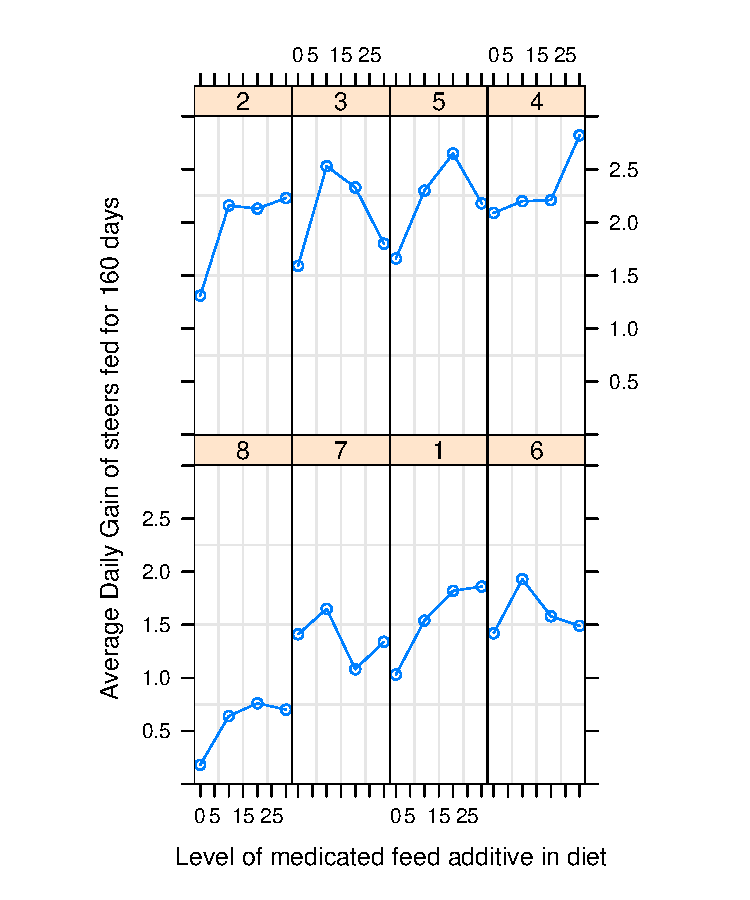
\includegraphics{figs/f-adg1}
  \caption{Average daily weight gain}
  \label{fig:adg1}
\end{figure}
\begin{Schunk}
\begin{Sinput}
> fm1Adg <- lme(adg ~ (Treatment - 1) * InitWt, data = AvgDailyGain, 
+     random = ~1 | Block)
> summary(fm1Adg)
\end{Sinput}
\begin{Soutput}
Linear mixed-effects model fit by REML
Fixed: adg ~ (Treatment - 1) * InitWt 
 Data: AvgDailyGain 
      AIC     BIC    logLik
 85.32685 99.9842 -32.66342

Random effects:
 Groups   Name        Variance Std.Dev.
 Block    (Intercept) 0.259311 0.50923 
 Residual             0.049429 0.22233 
# of obs: 32, groups: Block, 8

Fixed effects:
                     Estimate Std. Error DF t value Pr(>|t|)  
Treatment0          0.4391368  0.7110882 24  0.6176  0.54268  
Treatment10         1.4261185  0.6375459 24  2.2369  0.03485 *
Treatment20         0.4796283  0.5488868 24  0.8738  0.39088  
Treatment30         0.2001073  0.7751990 24  0.2581  0.79850  
InitWt              0.0044480  0.0020816 24  2.1368  0.04301 *
Treatment0:InitWt  -0.0021543  0.0027863 24 -0.7732  0.44695  
Treatment10:InitWt -0.0033651  0.0025148 24 -1.3381  0.19340  
Treatment20:InitWt -0.0010823  0.0024875 24 -0.4351  0.66737  
---
Signif. codes:  0 `***' 0.001 `**' 0.01 `*' 0.05 `.' 0.1 ` ' 1 

Correlation of Fixed Effects:
            Trtmn0 Trtm10 Trtm20 Trtm30 InitWt Tr0:IW T10:IW
Treatment10  0.039                                          
Treatment20  0.080  0.334                                   
Treatment30  0.011  0.097  0.043                            
InitWt       0.050 -0.032  0.035 -0.967                     
Trtmnt0:InW -0.640  0.046 -0.024  0.754 -0.780              
Trtmnt10:IW -0.021 -0.534 -0.178  0.781 -0.808  0.617       
Trtmnt20:IW -0.040 -0.106 -0.512  0.828 -0.856  0.666  0.775
\end{Soutput}
\begin{Sinput}
> anova(fm1Adg)
\end{Sinput}
\begin{Soutput}
Analysis of Variance Table
                 Df  Sum Sq Mean Sq   Denom F value    Pr(>F)    
Treatment         4  5.7248  1.4312 24.0000 28.9543 7.159e-09 ***
InitWt            1  0.5495  0.5495 24.0000 11.1175   0.00277 ** 
Treatment:InitWt  3  0.1381  0.0460 24.0000  0.9312   0.44088    
---
Signif. codes:  0 `***' 0.001 `**' 0.01 `*' 0.05 `.' 0.1 ` ' 1 
\end{Soutput}
\begin{Sinput}
> fm2Adg <- update(fm1Adg, adg ~ InitWt + Treatment)
> summary(fm2Adg)
\end{Sinput}
\begin{Soutput}
Linear mixed-effects model fit by REML
Fixed: adg ~ InitWt + Treatment 
 Data: AvgDailyGain 
      AIC      BIC    logLik
 50.33733 60.59748 -18.16866

Random effects:
 Groups   Name        Variance Std.Dev.
 Block    (Intercept) 0.24084  0.49076 
 Residual             0.05008  0.22379 
# of obs: 32, groups: Block, 8

Fixed effects:
               Estimate  Std. Error DF t value  Pr(>|t|)    
(Intercept)  0.80110842  0.35566103 27  2.2524  0.032628 *  
InitWt       0.00277971  0.00083335 27  3.3356  0.002486 ** 
Treatment0  -0.55207364  0.11481306 27 -4.8085 5.096e-05 ***
Treatment10 -0.06856608  0.11896892 27 -0.5763  0.569162    
Treatment20 -0.08812909  0.11628776 27 -0.7579  0.455103    
---
Signif. codes:  0 `***' 0.001 `**' 0.01 `*' 0.05 `.' 0.1 ` ' 1 

Correlation of Fixed Effects:
            (Intr) InitWt Trtmn0 Trtm10
InitWt      -0.844                     
Treatment0   0.036 -0.224              
Treatment10  0.139 -0.340  0.534       
Treatment20  0.079 -0.272  0.530  0.545
\end{Soutput}
\begin{Sinput}
> anova(fm2Adg)
\end{Sinput}
\begin{Soutput}
Analysis of Variance Table
          Df  Sum Sq Mean Sq   Denom F value    Pr(>F)    
InitWt     1  0.5146  0.5146 27.0000  10.275 0.0034525 ** 
Treatment  3  1.5267  0.5089 27.0000  10.162 0.0001185 ***
---
Signif. codes:  0 `***' 0.001 `**' 0.01 `*' 0.05 `.' 0.1 ` ' 1 
\end{Soutput}
\begin{Sinput}
> summary(update(fm1Adg, adg ~ InitWt + Treatment - 1))
\end{Sinput}
\begin{Soutput}
Linear mixed-effects model fit by REML
Fixed: adg ~ InitWt + Treatment - 1 
 Data: AvgDailyGain 
      AIC      BIC    logLik
 50.33733 60.59748 -18.16866

Random effects:
 Groups   Name        Variance Std.Dev.
 Block    (Intercept) 0.24084  0.49076 
 Residual             0.05008  0.22379 
# of obs: 32, groups: Block, 8

Fixed effects:
              Estimate Std. Error DF t value Pr(>|t|)   
InitWt      2.7797e-03 8.3335e-04 27  3.3356 0.002486 **
Treatment0  2.4903e-01 3.7763e-01 27  0.6595 0.515183   
Treatment10 7.3254e-01 3.9038e-01 27  1.8765 0.071437 . 
Treatment20 7.1298e-01 3.8277e-01 27  1.8627 0.073420 . 
Treatment30 8.0111e-01 3.5566e-01 27  2.2524 0.032628 * 
---
Signif. codes:  0 `***' 0.001 `**' 0.01 `*' 0.05 `.' 0.1 ` ' 1 

Correlation of Fixed Effects:
            InitWt Trtmn0 Trtm10 Trtm20
Treatment0  -0.863                     
Treatment10 -0.873  0.957              
Treatment20 -0.867  0.957  0.958       
Treatment30 -0.844  0.953  0.953  0.953
\end{Soutput}
\end{Schunk}


\section{BIB}
\label{sec:BIB}

A balanced incomplete, blocked design.  Compare with output 5.7
(p.~188) and output 5.9 (p.~193).
\begin{Schunk}
\begin{Sinput}
> print(gplot(BIB))
\end{Sinput}
\end{Schunk}
\begin{figure}[tbp]
  \centering
  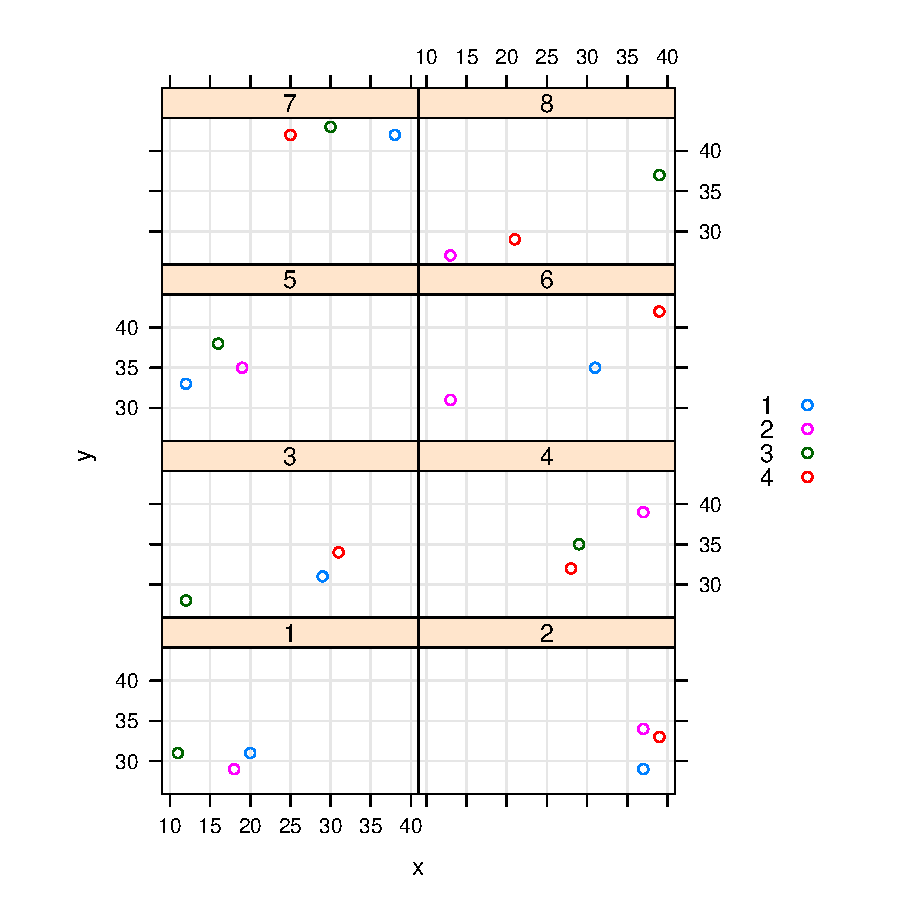
\includegraphics{figs/f-bib1}
  \caption{Balanced incomplete block design}
  \label{fig:bib1}
\end{figure}
\begin{Schunk}
\begin{Sinput}
> fm1BIB <- lme(y ~ Treatment * x, data = BIB, random = ~1 | 
+     Block)
> summary(fm1BIB)
\end{Sinput}
\begin{Soutput}
Linear mixed-effects model fit by REML
Fixed: y ~ Treatment * x 
 Data: BIB 
      AIC     BIC    logLik
 124.8945 136.675 -52.44723

Random effects:
 Groups   Name        Variance Std.Dev.
 Block    (Intercept) 18.2494  4.2719  
 Residual              1.2004  1.0956  
# of obs: 24, groups: Block, 8

Fixed effects:
              Estimate Std. Error DF t value  Pr(>|t|)    
(Intercept)  22.367853   3.101833 16  7.2112 2.075e-06 ***
Treatment1    4.429485   3.365069 16  1.3163 0.2066152    
Treatment2   -0.437371   2.933224 16 -0.1491 0.8833305    
Treatment3    6.278627   3.282059 16  1.9130 0.0738148 .  
x             0.442547   0.087063 16  5.0831 0.0001107 ***
Treatment1:x -0.223765   0.106083 16 -2.1093 0.0510220 .  
Treatment2:x  0.053384   0.097143 16  0.5495 0.5902247    
Treatment3:x -0.179177   0.115710 16 -1.5485 0.1410542    
---
Signif. codes:  0 `***' 0.001 `**' 0.01 `*' 0.05 `.' 0.1 ` ' 1 

Correlation of Fixed Effects:
            (Intr) Trtmn1 Trtmn2 Trtmn3 x      Trtm1: Trtm2:
Treatment1  -0.728                                          
Treatment2  -0.778  0.797                                   
Treatment3  -0.796  0.827  0.826                            
x           -0.859  0.797  0.865  0.886                     
Treatmnt1:x  0.709 -0.979 -0.774 -0.797 -0.799              
Treatmnt2:x  0.722 -0.731 -0.965 -0.763 -0.829  0.729       
Treatmnt3:x  0.769 -0.789 -0.790 -0.976 -0.879  0.777  0.748
\end{Soutput}
\begin{Sinput}
> anova(fm1BIB)
\end{Sinput}
\begin{Soutput}
Analysis of Variance Table
            Df  Sum Sq Mean Sq   Denom  F value    Pr(>F)    
Treatment    3  23.447   7.816  16.000   6.5108  0.004367 ** 
x            1 136.809 136.809  16.000 113.9669 1.098e-08 ***
Treatment:x  3  18.427   6.142  16.000   5.1167  0.011347 *  
---
Signif. codes:  0 `***' 0.001 `**' 0.01 `*' 0.05 `.' 0.1 ` ' 1 
\end{Soutput}
\begin{Sinput}
> fm2BIB <- lme(y ~ Treatment + x:Grp, data = BIB, random = ~1 | 
+     Block)
> summary(fm2BIB)
\end{Sinput}
\begin{Soutput}
Linear mixed-effects model fit by REML
Fixed: y ~ Treatment + x:Grp 
 Data: BIB 
      AIC      BIC    logLik
 115.1770 124.6015 -49.58851

Random effects:
 Groups   Name        Variance Std.Dev.
 Block    (Intercept) 18.5255  4.3041  
 Residual              1.0378  1.0187  
# of obs: 24, groups: Block, 8

Fixed effects:
             Estimate Std. Error DF t value  Pr(>|t|)    
(Intercept) 20.945165   2.062297 18 10.1562 7.032e-09 ***
Treatment1   5.341445   1.975705 18  2.7036 0.0145412 *  
Treatment2   1.135569   0.713988 18  1.5905 0.1291410    
Treatment3   8.181034   1.770100 18  4.6218 0.0002119 ***
x:Grp13      0.239520   0.042964 18  5.5750 2.722e-05 ***
x:Grp24      0.489230   0.044122 18 11.0882 1.781e-09 ***
---
Signif. codes:  0 `***' 0.001 `**' 0.01 `*' 0.05 `.' 0.1 ` ' 1 

Correlation of Fixed Effects:
           (Intr) Trtmn1 Trtmn2 Trtmn3 x:Gr13
Treatment1 -0.501                            
Treatment2 -0.431  0.559                     
Treatment3 -0.527  0.942  0.581              
x:Grp13     0.027 -0.663 -0.165 -0.605       
x:Grp24    -0.639  0.651  0.452  0.688  0.042
\end{Soutput}
\begin{Sinput}
> anova(fm2BIB)
\end{Sinput}
\begin{Soutput}
Analysis of Variance Table
          Df  Sum Sq Mean Sq   Denom F value    Pr(>F)    
Treatment  3  23.424   7.808  18.000  7.5235  0.001818 ** 
x:Grp      2 154.733  77.367  18.000 74.5468 1.954e-09 ***
---
Signif. codes:  0 `***' 0.001 `**' 0.01 `*' 0.05 `.' 0.1 ` ' 1 
\end{Soutput}
\end{Schunk}


\section{Bond}
\label{sec:Bond}

Compare with output 1.1 (p.~6).
\begin{Schunk}
\begin{Sinput}
> fm1Bond <- lme(pressure ~ Metal, data = Bond, random = ~1 | 
+     Ingot)
> summary(fm1Bond)
\end{Sinput}
\begin{Soutput}
Linear mixed-effects model fit by REML
Fixed: pressure ~ Metal 
 Data: Bond 
      AIC      BIC   logLik
 117.7902 123.0128 -53.8951

Random effects:
 Groups   Name        Variance Std.Dev.
 Ingot    (Intercept) 11.448   3.3835  
 Residual             10.372   3.2205  
# of obs: 21, groups: Ingot, 7

Fixed effects:
            Estimate Std. Error DF t value Pr(>|t|)    
(Intercept) 71.10000    1.76552 18 40.2715  < 2e-16 ***
Metalc      -0.91429    1.72143 18 -0.5311  0.60183    
Metali       4.80000    1.72143 18  2.7884  0.01213 *  
---
Signif. codes:  0 `***' 0.001 `**' 0.01 `*' 0.05 `.' 0.1 ` ' 1 

Correlation of Fixed Effects:
       (Intr) Metalc
Metalc -0.488       
Metali -0.488  0.500
\end{Soutput}
\begin{Sinput}
> anova(fm1Bond)
\end{Sinput}
\begin{Soutput}
Analysis of Variance Table
      Df Sum Sq Mean Sq  Denom F value   Pr(>F)   
Metal  2 131.90   65.95  18.00  6.3588 0.008147 **
---
Signif. codes:  0 `***' 0.001 `**' 0.01 `*' 0.05 `.' 0.1 ` ' 1 
\end{Soutput}
\end{Schunk}

\section{Cultivation}
\label{sec:Cultivation}

\begin{Schunk}
\begin{Sinput}
> print(bwplot(Cult ~ drywt | Block, Cultivation, layout = c(1, 
+     4)))
\end{Sinput}
\end{Schunk}
\begin{figure}[tbp]
  \centering
  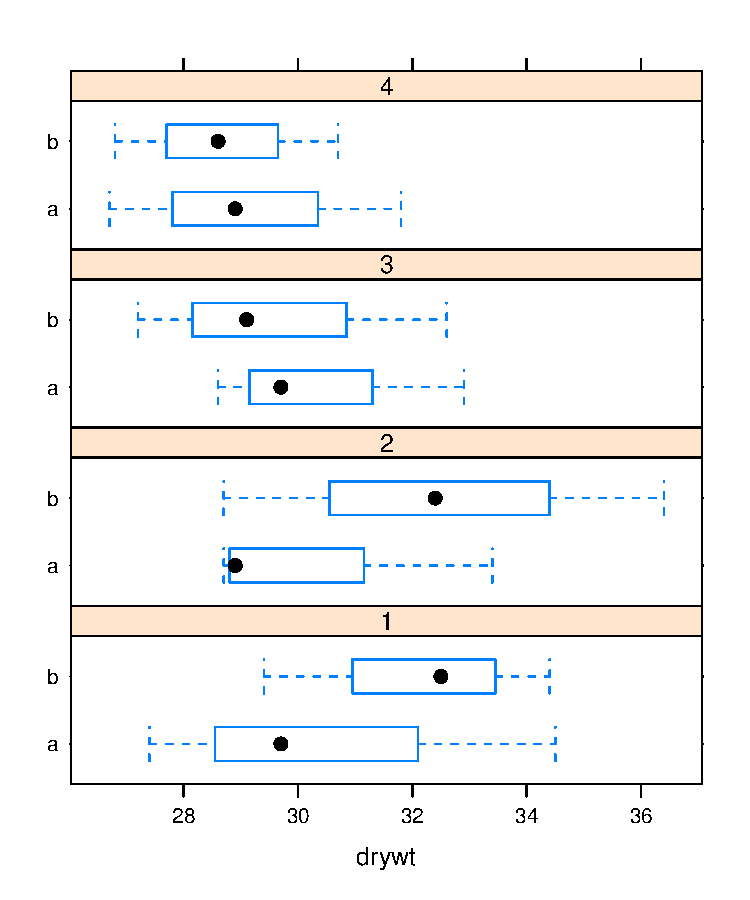
\includegraphics{figs/f-cult1}
  \caption{Cultivation data}
  \label{fig:adg1}
\end{figure}

A blocked split-plot design.  Compare these results with output 2.10 (p. 58).

\begin{Schunk}
\begin{Sinput}
> str(Cultivation)
\end{Sinput}
\begin{Soutput}
`data.frame':	24 obs. of  4 variables:
 $ Block: Factor w/ 4 levels "1","2","3","4": 1 1 1 1 1 1 2 2 2 2 ...
 $ Cult : Factor w/ 2 levels "a","b": 1 1 1 2 2 2 1 1 1 2 ...
 $ Inoc : Factor w/ 3 levels "con","dea","liv": 1 2 3 1 2 3 1 2 3 1 ...
 $ drywt: num  27.4 29.7 34.5 29.4 32.5 34.4 28.9 28.7 33.4 28.7 ...
 - attr(*, "ginfo")=List of 7
  ..$ formula     :Class 'formula' length 3 drywt ~ 1 | Block/Cult
  .. .. ..- attr(*, ".Environment")=length 6 <environment> 
  ..$ order.groups:List of 2
  .. ..$ Block: logi TRUE
  .. ..$ Cult : logi TRUE
  ..$ FUN         :function (x)  
  ..$ outer       : NULL
  ..$ inner       :List of 1
  .. ..$ Cult:Class 'formula' length 2 ~Inoc
  .. .. .. ..- attr(*, ".Environment")=length 6 <environment> 
  ..$ labels      :List of 1
  .. ..$ drywt: chr "Yield"
  ..$ units       : list()
\end{Soutput}
\begin{Sinput}
> xtabs(~Block + Cult, Cultivation)
\end{Sinput}
\begin{Soutput}
     Cult
Block a b
    1 3 3
    2 3 3
    3 3 3
    4 3 3
\end{Soutput}
\begin{Sinput}
> fm1Cult <- lme(drywt ~ Inoc * Cult, data = Cultivation, random = list(Block = ~1, 
+     Cult = ~1))
> summary(fm1Cult)
\end{Sinput}
\begin{Soutput}
Linear mixed-effects model fit by REML
Fixed: drywt ~ Inoc * Cult 
 Data: Cultivation 
      AIC     BIC    logLik
 86.48742 97.0899 -34.24371

Random effects:
 Groups   Name        Variance Std.Dev.
 Block    (Intercept) 1.20728  1.09876 
 Cult     (Intercept) 0.26585  0.51561 
 Residual             1.19633  1.09377 
# of obs: 24, groups: Block, 4; Cult, 2

Fixed effects:
              Estimate Std. Error DF t value  Pr(>|t|)    
(Intercept)   33.52500    0.93100 18 36.0098 < 2.2e-16 ***
Inoccon       -5.50000    0.77341 18 -7.1113 1.256e-06 ***
Inocdea       -2.87500    0.77341 18 -3.7173  0.001577 ** 
Culta         -0.37500    1.06295 18 -0.3528  0.728343    
Inoccon:Culta  0.25000    1.09377 18  0.2286  0.821782    
Inocdea:Culta -1.02500    1.09377 18 -0.9371  0.361098    
---
Signif. codes:  0 `***' 0.001 `**' 0.01 `*' 0.05 `.' 0.1 ` ' 1 

Correlation of Fixed Effects:
            (Intr) Inoccn Inocde Culta  Incc:C
Inoccon     -0.415                            
Inocdea     -0.415  0.500                     
Culta       -0.571  0.364  0.364              
Inoccon:Clt  0.294 -0.707 -0.354 -0.514       
Inocdea:Clt  0.294 -0.354 -0.707 -0.514  0.500
\end{Soutput}
\begin{Sinput}
> anova(fm1Cult)
\end{Sinput}
\begin{Soutput}
Analysis of Variance Table
          Df  Sum Sq Mean Sq   Denom F value   Pr(>F)    
Inoc       2 118.176  59.088  18.000 49.3909 4.91e-08 ***
Cult       1   0.656   0.656  18.000  0.5486   0.4684    
Inoc:Cult  2   1.826   0.913  18.000  0.7631   0.4807    
---
Signif. codes:  0 `***' 0.001 `**' 0.01 `*' 0.05 `.' 0.1 ` ' 1 
\end{Soutput}
\begin{Sinput}
> fm2Cult <- update(fm1Cult, drywt ~ Inoc + Cult)
> anova(fm2Cult)
\end{Sinput}
\begin{Soutput}
Analysis of Variance Table
     Df  Sum Sq Mean Sq   Denom F value    Pr(>F)    
Inoc  2 118.176  59.088  20.000 50.8069 1.447e-08 ***
Cult  1   0.656   0.656  20.000  0.5644    0.4613    
---
Signif. codes:  0 `***' 0.001 `**' 0.01 `*' 0.05 `.' 0.1 ` ' 1 
\end{Soutput}
\begin{Sinput}
> fm3Cult <- update(fm1Cult, drywt ~ Inoc)
> anova(fm3Cult)
\end{Sinput}
\begin{Soutput}
Analysis of Variance Table
     Df  Sum Sq Mean Sq   Denom F value    Pr(>F)    
Inoc  2 118.176  59.088  21.000  50.807 8.988e-09 ***
---
Signif. codes:  0 `***' 0.001 `**' 0.01 `*' 0.05 `.' 0.1 ` ' 1 
\end{Soutput}
\begin{Sinput}
> summary(fm3Cult)
\end{Sinput}
\begin{Soutput}
Linear mixed-effects model fit by REML
Fixed: drywt ~ Inoc 
 Data: Cultivation 
      AIC      BIC    logLik
 87.67784 94.74616 -37.83892

Random effects:
 Groups   Name        Variance Std.Dev.
 Block    (Intercept) 1.21283  1.10129 
 Cult     (Intercept) 0.10364  0.32193 
 Residual             1.16299  1.07842 
# of obs: 24, groups: Block, 4; Cult, 2

Fixed effects:
            Estimate Std. Error DF t value  Pr(>|t|)    
(Intercept) 33.33750    0.70739 21 47.1275 < 2.2e-16 ***
Inoccon     -5.37500    0.53921 21 -9.9683 2.048e-09 ***
Inocdea     -3.38750    0.53921 21 -6.2823 3.134e-06 ***
---
Signif. codes:  0 `***' 0.001 `**' 0.01 `*' 0.05 `.' 0.1 ` ' 1 

Correlation of Fixed Effects:
        (Intr) Inoccn
Inoccon -0.381       
Inocdea -0.381  0.500
\end{Soutput}
\end{Schunk}

A blocked split-plot with missing data (sec 2.7, pp. 68-75).  The data
in Block 1 and Cultivar 'a' are removed from the data set

\begin{Schunk}
\begin{Sinput}
> CultMiss <- Cultivation[Cultivation$Block != 1 | Cultivation$Cult != 
+     "a", ]
> dim(CultMiss)
\end{Sinput}
\begin{Soutput}
[1] 21  4
\end{Soutput}
\end{Schunk}
\begin{Schunk}
\begin{Sinput}
> print(bwplot(Cult ~ drywt | Block, CultMiss, layout = c(1, 
+     4)))
\end{Sinput}
\end{Schunk}
\begin{figure}[tbp]
  \centering
  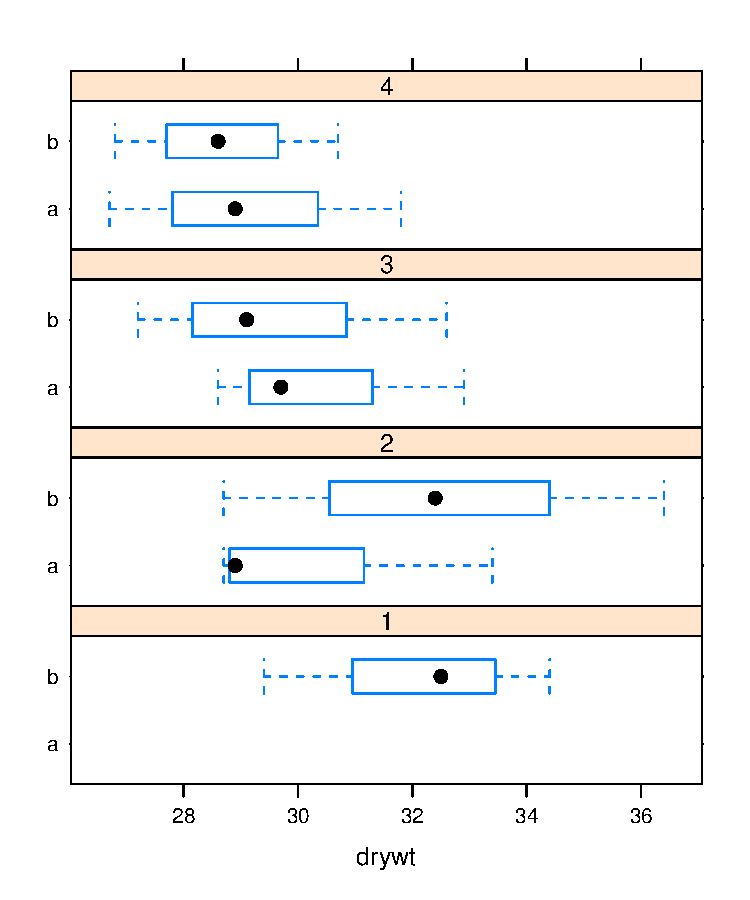
\includegraphics{figs/f-cultm1}
  \caption{Cultivation data with missing cell}
  \label{fig:adg1}
\end{figure}

\begin{Schunk}
\begin{Sinput}
> fm1CultM <- lme(drywt ~ Cult * Inoc, CultMiss, list(Block = ~1, 
+     Cult = ~1), method = "ML")
> summary(fm1CultM)
\end{Sinput}
\begin{Soutput}
Linear mixed-effects model fit by maximum likelihood
Fixed: drywt ~ Cult * Inoc 
 Data: CultMiss 
      AIC      BIC    logLik
 81.96929 91.36999 -31.98464

Random effects:
 Groups   Name        Variance   Std.Dev.  
 Block    (Intercept) 1.1906e+00 1.0911e+00
 Cult     (Intercept) 8.2202e-11 9.0666e-06
 Residual             8.2202e-01 9.0666e-01
# of obs: 21, groups: Block, 4; Cult, 2

Fixed effects:
              Estimate Std. Error DF t value  Pr(>|t|)    
(Intercept)   33.52500    0.70934 15 47.2625 < 2.2e-16 ***
Culta         -0.45467    0.70575 15 -0.6442 0.5291462    
Inoccon       -5.50000    0.64110 15 -8.5790 3.604e-07 ***
Inocdea       -2.87500    0.64110 15 -4.4845 0.0004366 ***
Culta:Inoccon  0.86667    0.97930 15  0.8850 0.3901303    
Culta:Inocdea -0.72500    0.97930 15 -0.7403 0.4705331    
---
Signif. codes:  0 `***' 0.001 `**' 0.01 `*' 0.05 `.' 0.1 ` ' 1 

Correlation of Fixed Effects:
            (Intr) Culta  Inoccn Inocde Clt:Incc
Culta       -0.411                              
Inoccon     -0.452  0.454                       
Inocdea     -0.452  0.454  0.500                
Culta:Inccn  0.296 -0.694 -0.655 -0.327         
Culta:Inocd  0.296 -0.694 -0.327 -0.655  0.500  
\end{Soutput}
\begin{Sinput}
> fm2CultM <- update(fm1CultM, drywt ~ Cult + Inoc)
> fm3CultM <- update(fm1CultM, drywt ~ Inoc)
> fm4CultM <- update(fm1CultM, drywt ~ 1)
> anova(fm1CultM, fm2CultM, fm3CultM, fm4CultM)
\end{Sinput}
\begin{Soutput}
Data: CultMiss

Models: <fixed>: <random>
fm4CultM: drywt ~ 1: list(Block = ~1, Cult = ~1)
fm3CultM: drywt ~ Inoc: list(Block = ~1, Cult = ~1)
fm2CultM: drywt ~ Cult + Inoc: list(Block = ~1, Cult = ~1)
fm1CultM: drywt ~ Cult * Inoc: list(Block = ~1, Cult = ~1)

         Df     AIC     BIC  logLik   Chisq Chi Df Pr(>Chisq)    
fm4CultM  4 107.333 111.511 -49.667                              
fm3CultM  6  79.263  85.531 -33.632 32.0696      2  1.087e-07 ***
fm2CultM  7  80.430  87.741 -33.215  0.8340      1     0.3611    
fm1CultM  9  81.969  91.370 -31.985  2.4602      2     0.2923    
---
Signif. codes:  0 `***' 0.001 `**' 0.01 `*' 0.05 `.' 0.1 ` ' 1 
\end{Soutput}
\begin{Sinput}
> fm3RCultM <- update(fm3CultM, method = "REML")
> summary(fm3RCultM)
\end{Sinput}
\begin{Soutput}
Linear mixed-effects model fit by REML
Fixed: drywt ~ Inoc 
 Data: CultMiss 
      AIC      BIC    logLik
 77.31883 83.58596 -32.65941

Random effects:
 Groups   Name        Variance   Std.Dev.  
 Block    (Intercept) 1.7626e+00 1.3276e+00
 Cult     (Intercept) 1.1064e-10 1.0518e-05
 Residual             1.1064e+00 1.0518e+00
# of obs: 21, groups: Block, 4; Cult, 2

Fixed effects:
            Estimate Std. Error DF t value  Pr(>|t|)    
(Intercept) 33.35105    0.77645 18 42.9532 < 2.2e-16 ***
Inoccon     -5.12857    0.56223 18 -9.1218 3.604e-08 ***
Inocdea     -3.18571    0.56223 18 -5.6662 2.249e-05 ***
---
Signif. codes:  0 `***' 0.001 `**' 0.01 `*' 0.05 `.' 0.1 ` ' 1 

Correlation of Fixed Effects:
        (Intr) Inoccn
Inoccon -0.362       
Inocdea -0.362  0.500
\end{Soutput}
\end{Schunk}

\section{Demand}
\label{sec:Demand}

\begin{Schunk}
\begin{Sinput}
> print(gplot(Demand, scales = list(y = list(log = 2))))
\end{Sinput}
\end{Schunk}
\begin{figure}[tbp]
  \centering
  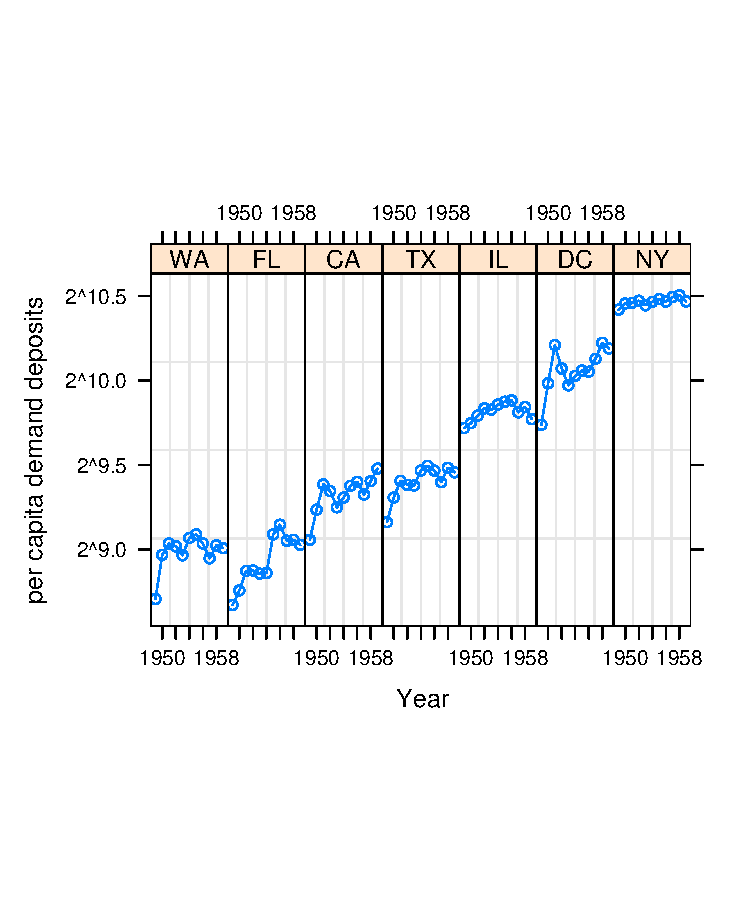
\includegraphics{figs/f-demand1}
  \caption{Per-capita demand deposits versus year by state.  The
    vertical axis is on a logarithmic scale.}
  \label{fig:demand1}
\end{figure}
Analysis of the per capita demand deposits data given as data set 3.6.
Compare these results with output 3.13 (p.~132).

Notice that although \code{Year} is stored numerically, it is
converted to a factor when used as a grouping factor.
\begin{Schunk}
\begin{Sinput}
> str(Demand)
\end{Sinput}
\begin{Soutput}
`data.frame':	77 obs. of  7 variables:
 $ State: Factor w/ 7 levels "CA","DC","FL",..: 1 1 1 1 1 1 1 1 1 1 ...
 $ Year : num  1949 1950 1951 1952 1953 ...
 $ d    : num  533 603 669 651 609 634 665 676 642 678 ...
 $ y    : num  1347 1464 1608 1636 1669 ...
 $ rd   : num  0.343 0.364 0.367 0.369 0.41 0.499 0.496 0.533 0.63 0.667 ...
 $ rt   : num  1.11 1.16 1.49 1.57 1.59 ...
 $ rs   : num  2.90 2.94 3.09 3.07 3.36 ...
 - attr(*, "ginfo")=List of 7
  ..$ formula     :Class 'formula' length 3 d ~ Year | State
  .. .. ..- attr(*, ".Environment")=length 15 <environment> 
  ..$ order.groups: logi TRUE
  ..$ FUN         :function (x)  
  ..$ outer       : NULL
  ..$ inner       : NULL
  ..$ labels      :List of 1
  .. ..$ d: chr "per capita demand deposits"
  ..$ units       : list()
\end{Soutput}
\begin{Sinput}
> fm1Demand <- lme(log(d) ~ log(y) + log(rd) + log(rt) + log(rs), 
+     Demand, ~1 | State + Year)
> summary(fm1Demand)
\end{Sinput}
\begin{Soutput}
Linear mixed-effects model fit by REML
Fixed: log(d) ~ log(y) + log(rd) + log(rt) + log(rs) 
 Data: Demand 
       AIC       BIC   logLik
 -224.1653 -205.4148 120.0826

Random effects:
 Groups   Name        Variance   Std.Dev.
 Year     (Intercept) 0.00026465 0.016268
 State    (Intercept) 0.02948900 0.171724
 Residual             0.00111705 0.033422
# of obs: 77, groups: Year, 11; State, 7

Fixed effects:
             Estimate Std. Error DF t value  Pr(>|t|)    
(Intercept) -1.284043   0.723423 72 -1.7750  0.080132 .  
log(y)       1.069806   0.103925 72 10.2941 8.553e-16 ***
log(rd)     -0.295342   0.052463 72 -5.6296 3.265e-07 ***
log(rt)      0.039882   0.027889 72  1.4300  0.157034    
log(rs)     -0.326739   0.114385 72 -2.8565  0.005595 ** 
---
Signif. codes:  0 `***' 0.001 `**' 0.01 `*' 0.05 `.' 0.1 ` ' 1 

Correlation of Fixed Effects:
        (Intr) log(y) lg(rd) lg(rt)
log(y)  -0.976                     
log(rd)  0.383 -0.227              
log(rt)  0.077 -0.062 -0.337       
log(rs)  0.444 -0.600 -0.270 -0.323
\end{Soutput}
\end{Schunk}

\section{Genetics}
\label{sec:Genetics}

Analysis of the heritability data given as data set 4.5.  To obtain a
term for the location/family interaction we must create a separate
grouping factor.  Similarly for the Block within Location.
\begin{Schunk}
\begin{Sinput}
> Genetics$LocFam <- with(Genetics, Location:Family)
> Genetics$LocBloc <- with(Genetics, Location:Block)
> fm1Gen <- lme(Yield ~ 1, Genetics, ~1 | LocFam + LocBloc + 
+     Family + Location)
> summary(fm1Gen)
\end{Sinput}
\begin{Soutput}
Linear mixed-effects model fit by REML
Fixed: Yield ~ 1 
 Data: Genetics 
      AIC      BIC    logLik
 485.9865 498.5525 -236.9932

Random effects:
 Groups   Name        Variance Std.Dev.
 LocFam   (Intercept)  74.861   8.6523 
 LocBloc  (Intercept)  89.325   9.4512 
 Family   (Intercept) 187.857  13.7061 
 Location (Intercept) 612.945  24.7577 
 Residual              51.854   7.2010 
# of obs: 60, groups: LocFam, 20; LocBloc, 12; Family, 5; Location, 4

Fixed effects:
            Estimate Std. Error DF t value  Pr(>|t|)    
(Intercept)  209.133     14.243 59  14.683 < 2.2e-16 ***
---
Signif. codes:  0 `***' 0.001 `**' 0.01 `*' 0.05 `.' 0.1 ` ' 1 
\end{Soutput}
\begin{Sinput}
> summary(fm2Gen <- lme(Yield ~ Family, Genetics, ~1 | LocFam + 
+     LocBloc + Location))
\end{Sinput}
\begin{Soutput}
Linear mixed-effects model fit by REML
Fixed: Yield ~ Family 
 Data: Genetics 
      AIC      BIC    logLik
 457.6174 476.4665 -219.8087

Random effects:
 Groups   Name        Variance Std.Dev.
 LocFam   (Intercept)  74.861   8.6522 
 LocBloc  (Intercept)  89.322   9.4510 
 Location (Intercept) 613.082  24.7605 
 Residual              51.850   7.2007 
# of obs: 60, groups: LocFam, 20; LocBloc, 12; Location, 4

Fixed effects:
            Estimate Std. Error DF t value  Pr(>|t|)    
(Intercept) 207.4167    13.5554 55 15.3014 < 2.2e-16 ***
Family1      22.1667     6.7876 55  3.2657  0.001882 ** 
Family2       9.0833     6.7876 55  1.3382  0.186332    
Family3     -15.0833     6.7876 55 -2.2222  0.030403 *  
Family4      -7.5833     6.7876 55 -1.1172  0.268754    
---
Signif. codes:  0 `***' 0.001 `**' 0.01 `*' 0.05 `.' 0.1 ` ' 1 

Correlation of Fixed Effects:
        (Intr) Famly1 Famly2 Famly3
Family1 -0.250                     
Family2 -0.250  0.500              
Family3 -0.250  0.500  0.500       
Family4 -0.250  0.500  0.500  0.500
\end{Soutput}
\begin{Sinput}
> summary(fm3Gen <- lme(Yield ~ Family, Genetics, ~1 | LocBloc + 
+     Location))
\end{Sinput}
\begin{Soutput}
Linear mixed-effects model fit by REML
Fixed: Yield ~ Family 
 Data: Genetics 
      AIC      BIC    logLik
 469.8516 486.6063 -226.9258

Random effects:
 Groups   Name        Variance Std.Dev.
 LocBloc  (Intercept)  77.07    8.779  
 Location (Intercept) 628.64   25.073  
 Residual             113.10   10.635  
# of obs: 60, groups: LocBloc, 12; Location, 4

Fixed effects:
            Estimate Std. Error DF t value  Pr(>|t|)    
(Intercept) 207.4167    13.1532 55 15.7692 < 2.2e-16 ***
Family1      22.1667     4.3416 55  5.1057 4.246e-06 ***
Family2       9.0833     4.3416 55  2.0922  0.041052 *  
Family3     -15.0833     4.3416 55 -3.4742  0.001007 ** 
Family4      -7.5833     4.3416 55 -1.7467  0.086276 .  
---
Signif. codes:  0 `***' 0.001 `**' 0.01 `*' 0.05 `.' 0.1 ` ' 1 

Correlation of Fixed Effects:
        (Intr) Famly1 Famly2 Famly3
Family1 -0.165                     
Family2 -0.165  0.500              
Family3 -0.165  0.500  0.500       
Family4 -0.165  0.500  0.500  0.500
\end{Soutput}
\begin{Sinput}
> anova(fm2Gen, fm3Gen)
\end{Sinput}
\begin{Soutput}
Data: Genetics

Models: <fixed>: <random>
fm3Gen: Yield ~ Family: ~1 | LocBloc + Location
fm2Gen: Yield ~ Family: ~1 | LocFam + LocBloc + Location

       Df     AIC     BIC  logLik  Chisq Chi Df Pr(>Chisq)   
fm3Gen  8  494.51  511.27 -239.26                            
fm2Gen  9  485.85  504.70 -233.93 10.660      1   0.001095 **
---
Signif. codes:  0 `***' 0.001 `**' 0.01 `*' 0.05 `.' 0.1 ` ' 1 
\end{Soutput}
\end{Schunk}

\section{HR}
\label{sec:HR}
\begin{Schunk}
\begin{Sinput}
> print(gplot(HR))
\end{Sinput}
\end{Schunk}
\begin{figure}[tbp]
  \centering
  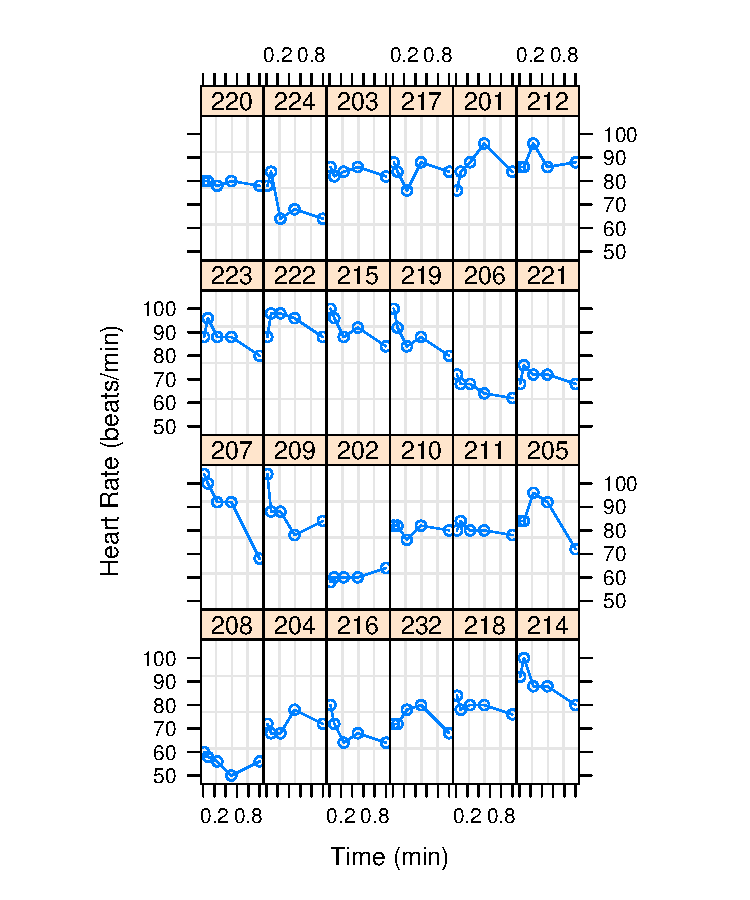
\includegraphics{figs/f-hr1}
  \caption{Heart rate data}
  \label{fig:hr1}
\end{figure}
Analysis of the Heart rate data given as data set 3.5.  Compare with
output 3.12 (pp.~128--129)
\begin{Schunk}
\begin{Sinput}
> fm1HR <- lme(HR ~ Time * Drug + baseHR, data = HR, random = ~Time | 
+     Patient)
> summary(fm1HR)
\end{Sinput}
\begin{Soutput}
Linear mixed-effects model fit by REML
Fixed: HR ~ Time * Drug + baseHR 
 Data: HR 
     AIC      BIC    logLik
 789.607 820.2694 -383.8035

Random effects:
 Groups   Name        Variance Std.Dev. Corr   
 Patient  (Intercept) 60.630   7.7866          
          Time        37.786   6.1470   -0.563 
 Residual             24.361   4.9357          
# of obs: 120, groups: Patient, 24

Fixed effects:
             Estimate Std. Error  DF t value  Pr(>|t|)    
(Intercept)  33.97835   10.28243 113  3.3045  0.001275 ** 
Time         -3.19704    3.08498 113 -1.0363  0.302263    
Druga         3.59915    4.23132 113  0.8506  0.396791    
Drugb         7.09121    4.20934 113  1.6846  0.094819 .  
baseHR        0.54342    0.11614 113  4.6789 8.058e-06 ***
Time:Druga   -7.50131    4.36282 113 -1.7194  0.088285 .  
Time:Drugb   -3.98942    4.36282 113 -0.9144  0.362447    
---
Signif. codes:  0 `***' 0.001 `**' 0.01 `*' 0.05 `.' 0.1 ` ' 1 

Correlation of Fixed Effects:
           (Intr) Time   Druga  Drugb  baseHR Tim:Drg
Time       -0.162                                    
Druga      -0.308  0.394                             
Drugb      -0.244  0.396  0.501                      
baseHR     -0.957  0.000  0.110  0.041               
Time:Druga  0.115 -0.707 -0.557 -0.280  0.000        
Time:Drugb  0.115 -0.707 -0.278 -0.560  0.000  0.500 
\end{Soutput}
\begin{Sinput}
> anova(fm1HR)
\end{Sinput}
\begin{Soutput}
Analysis of Variance Table
          Df Sum Sq Mean Sq  Denom F value    Pr(>F)    
Time       1 379.22  379.22 113.00 15.5665 0.0001387 ***
Drug       2  92.90   46.45 113.00  1.9067 0.1533252    
baseHR     1 533.32  533.32 113.00 21.8923 8.058e-06 ***
Time:Drug  2  72.11   36.06 113.00  1.4801 0.2319904    
---
Signif. codes:  0 `***' 0.001 `**' 0.01 `*' 0.05 `.' 0.1 ` ' 1 
\end{Soutput}
\begin{Sinput}
> fm3HR <- update(fm1HR, HR ~ Time + Drug + baseHR)
> anova(fm3HR)
\end{Sinput}
\begin{Soutput}
Analysis of Variance Table
       Df Sum Sq Mean Sq  Denom F value    Pr(>F)    
Time    1 364.03  364.03 115.00 14.9431 0.0001839 ***
Drug    2  92.88   46.44 115.00  1.9064 0.1532830    
baseHR  1 533.27  533.27 115.00 21.8905 7.937e-06 ***
---
Signif. codes:  0 `***' 0.001 `**' 0.01 `*' 0.05 `.' 0.1 ` ' 1 
\end{Soutput}
\begin{Sinput}
> summary(fm3HR)
\end{Sinput}
\begin{Soutput}
Linear mixed-effects model fit by REML
Fixed: HR ~ Time + Drug + baseHR 
 Data: HR 
      AIC      BIC    logLik
 797.8283 822.9158 -389.9142

Random effects:
 Groups   Name        Variance Std.Dev. Corr   
 Patient  (Intercept) 61.560   7.8460          
          Time        40.963   6.4002   -0.571 
 Residual             24.361   4.9357          
# of obs: 120, groups: Patient, 24

Fixed effects:
             Estimate Std. Error  DF t value  Pr(>|t|)    
(Intercept)  36.04640   10.19449 115  3.5359 0.0005868 ***
Time         -7.02729    1.81789 115 -3.8656 0.0001839 ***
Druga        -0.45237    3.51456 115 -0.1287 0.8978087    
Drugb         4.93648    3.48807 115  1.4152 0.1596980    
baseHR        0.54342    0.11615 115  4.6787 7.937e-06 ***
---
Signif. codes:  0 `***' 0.001 `**' 0.01 `*' 0.05 `.' 0.1 ` ' 1 

Correlation of Fixed Effects:
       (Intr) Time   Druga  Drugb 
Time   -0.096                     
Druga  -0.297  0.000              
Drugb  -0.219  0.000  0.502       
baseHR -0.966  0.000  0.132  0.050
\end{Soutput}
\begin{Sinput}
> fm4HR <- update(fm3HR, HR ~ Time + baseHR)
> anova(fm4HR)
\end{Sinput}
\begin{Soutput}
Analysis of Variance Table
       Df Sum Sq Mean Sq  Denom F value    Pr(>F)    
Time    1 364.03  364.03 117.00  14.943 0.0001825 ***
baseHR  1 534.87  534.87 117.00  21.956 7.593e-06 ***
---
Signif. codes:  0 `***' 0.001 `**' 0.01 `*' 0.05 `.' 0.1 ` ' 1 
\end{Soutput}
\begin{Sinput}
> summary(fm4HR)
\end{Sinput}
\begin{Soutput}
Linear mixed-effects model fit by REML
Fixed: HR ~ Time + baseHR 
 Data: HR 
      AIC      BIC    logLik
 805.1481 824.6605 -395.5740

Random effects:
 Groups   Name        Variance Std.Dev. Corr   
 Patient  (Intercept) 63.026   7.9389          
          Time        40.963   6.4002   -0.553 
 Residual             24.361   4.9357          
# of obs: 120, groups: Patient, 24

Fixed effects:
             Estimate Std. Error  DF t value  Pr(>|t|)    
(Intercept)  36.93141    9.90143 117  3.7299 0.0002969 ***
Time         -7.02729    1.81789 117 -3.8656 0.0001825 ***
baseHR        0.55078    0.11754 117  4.6857 7.593e-06 ***
---
Signif. codes:  0 `***' 0.001 `**' 0.01 `*' 0.05 `.' 0.1 ` ' 1 

Correlation of Fixed Effects:
       (Intr) Time  
Time   -0.098       
baseHR -0.984  0.000
\end{Soutput}
\end{Schunk}

\section{Mississippi}
\label{sec:Mississippi}
\begin{Schunk}
\begin{Sinput}
> print(gplot(Mississippi))
\end{Sinput}
\end{Schunk}

Analysis of the Mississippi nitrogren concentrations given as data set
4.2.  Compare with output 4.1 (p.~142), 4.2 (p.~143) up to output 4.9
(pp.~150--152). 
\begin{figure}[tbp]
  \centering
  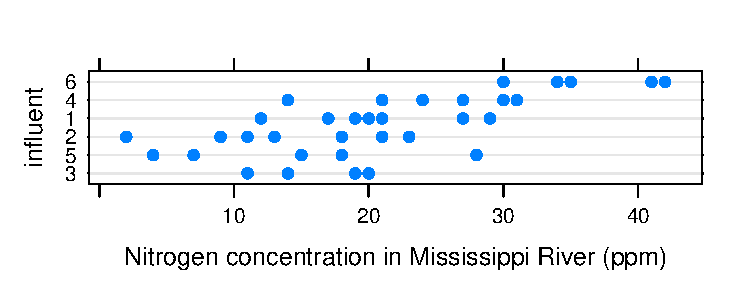
\includegraphics{figs/f-mississippi1}
  \caption{Heart rate data}
  \label{fig:mississippi1}
\end{figure}

\begin{Schunk}
\begin{Sinput}
> fm1Miss <- lme(y ~ 1, data = Mississippi, random = ~1 | influent)
> summary(fm1Miss)
\end{Sinput}
\begin{Soutput}
Linear mixed-effects model fit by REML
Fixed: y ~ 1 
 Data: Mississippi 
      AIC      BIC    logLik
 258.3511 263.1839 -126.1756

Random effects:
 Groups   Name        Variance Std.Dev.
 influent (Intercept) 63.323   7.9576  
 Residual             42.658   6.5313  
# of obs: 37, groups: influent, 6

Fixed effects:
            Estimate Std. Error DF t value  Pr(>|t|)    
(Intercept)   21.223      3.429 36  6.1892 3.885e-07 ***
---
Signif. codes:  0 `***' 0.001 `**' 0.01 `*' 0.05 `.' 0.1 ` ' 1 
\end{Soutput}
\begin{Sinput}
> fm1MLMiss <- update(fm1Miss, method = "ML")
> summary(fm1MLMiss)
\end{Sinput}
\begin{Soutput}
Linear mixed-effects model fit by maximum likelihood
Fixed: y ~ 1 
 Data: Mississippi 
     AIC      BIC    logLik
 262.557 267.3898 -128.2785

Random effects:
 Groups   Name        Variance Std.Dev.
 influent (Intercept) 51.255   7.1592  
 Residual             42.697   6.5343  
# of obs: 37, groups: influent, 6

Fixed effects:
            Estimate Std. Error DF t value  Pr(>|t|)    
(Intercept)   21.217      3.122 36   6.796 6.089e-08 ***
---
Signif. codes:  0 `***' 0.001 `**' 0.01 `*' 0.05 `.' 0.1 ` ' 1 
\end{Soutput}
\begin{Sinput}
> ranef(fm1MLMiss)
\end{Sinput}
\begin{Soutput}
$influent
  (Intercept)
1   0.3097833
2  -6.5772278
3  -3.7862748
4   2.8826711
5  -5.8435210
6  13.0145691
\end{Soutput}
\begin{Sinput}
> ranef(fm1Miss)
\end{Sinput}
\begin{Soutput}
$influent
  (Intercept)
1    0.309286
2   -6.719332
3   -3.897945
4    2.946104
5   -6.012984
6   13.374871
\end{Soutput}
\begin{Sinput}
> VarCorr(fm1Miss)
\end{Sinput}
\begin{Soutput}
 Groups   Name        Variance Std.Dev.
 influent (Intercept) 63.323   7.9576  
 Residual             42.658   6.5313  
\end{Soutput}
\begin{Sinput}
> fm2Miss <- lme(y ~ Type, data = Mississippi, random = ~1 | 
+     influent, method = "REML")
> summary(fm2Miss)
\end{Sinput}
\begin{Soutput}
Linear mixed-effects model fit by REML
Fixed: y ~ Type 
 Data: Mississippi 
      AIC      BIC    logLik
 244.5246 252.5792 -117.2623

Random effects:
 Groups   Name        Variance Std.Dev.
 influent (Intercept) 14.970   3.8691  
 Residual             42.514   6.5202  
# of obs: 37, groups: influent, 6

Fixed effects:
            Estimate Std. Error DF t value  Pr(>|t|)    
(Intercept)  36.4000     4.8449 34  7.5131 1.011e-08 ***
Type1       -20.8000     5.9338 34 -3.5054  0.001302 ** 
Type2       -16.4619     5.5168 34 -2.9840  0.005238 ** 
---
Signif. codes:  0 `***' 0.001 `**' 0.01 `*' 0.05 `.' 0.1 ` ' 1 

Correlation of Fixed Effects:
      (Intr) Type1 
Type1 -0.816       
Type2 -0.878  0.717
\end{Soutput}
\begin{Sinput}
> anova(fm2Miss)
\end{Sinput}
\begin{Soutput}
Analysis of Variance Table
     Df Sum Sq Mean Sq  Denom F value   Pr(>F)   
Type  2 541.76  270.88  34.00  6.3716 0.004466 **
---
Signif. codes:  0 `***' 0.001 `**' 0.01 `*' 0.05 `.' 0.1 ` ' 1 
\end{Soutput}
\end{Schunk}

\section{Multilocation}
\label{sec:Multilocation}

Analysis of the Multilocation data with fixed effects for the
locations.  We create a grouping factor for Block within Location and
for the Location/Treatment interaction.

\begin{Schunk}
\begin{Sinput}
> str(Multilocation)
\end{Sinput}
\begin{Soutput}
`data.frame':	108 obs. of  7 variables:
 $ obs     : num  3 4 6 7 9 10 12 16 19 20 ...
 $ Location: Factor w/ 9 levels "A","B","C","D",..: 1 1 1 1 1 1 1 1 1 1 ...
 $ Block   : Factor w/ 3 levels "1","2","3": 1 1 1 1 2 2 2 2 3 3 ...
 $ Trt     : Factor w/ 4 levels "1","2","3","4": 3 4 2 1 2 1 3 4 1 2 ...
 $ Adj     : num  3.16 3.12 3.16 3.25 2.71 ...
 $ Fe      : num  7.10 6.68 6.83 6.53 8.25 ...
 $ Grp     : Factor w/ 27 levels "A/1","A/2","A/3",..: 1 1 1 1 2 2 2 2 3 3 ...
 - attr(*, "ginfo")=List of 7
  ..$ formula     :Class 'formula' length 3 Adj ~ 1 | Location/Block
  .. .. ..- attr(*, ".Environment")=length 26 <environment> 
  ..$ order.groups:List of 2
  .. ..$ Location: logi TRUE
  .. ..$ Block   : logi TRUE
  ..$ FUN         :function (x)  
  ..$ outer       : NULL
  ..$ inner       :List of 1
  .. ..$ Block:Class 'formula' length 2 ~Trt
  .. .. .. ..- attr(*, ".Environment")=length 26 <environment> 
  ..$ labels      :List of 1
  .. ..$ Adj: chr "Adjusted yield"
  ..$ units       : list()
\end{Soutput}
\begin{Sinput}
> Multilocation$Grp <- with(Multilocation, Block:Location)[drop = TRUE]
> Multilocation$Int <- with(Multilocation, Location:Trt)[drop = TRUE]
> fm1Mult <- lme(Adj ~ Location * Trt, data = Multilocation, 
+     ~1 | Grp)
> summary(fm1Mult)
\end{Sinput}
\begin{Soutput}
Linear mixed-effects model fit by REML
Fixed: Adj ~ Location * Trt 
 Data: Multilocation 
      AIC      BIC    logLik
 86.64621 188.5672 -5.323106

Random effects:
 Groups   Name        Variance  Std.Dev.
 Grp      (Intercept) 0.0056193 0.074962
 Residual             0.0345787 0.185953
# of obs: 108, groups: Grp, 27

Fixed effects:
                Estimate Std. Error DF t value  Pr(>|t|)    
(Intercept)     2.359233   0.115755 72 20.3812 < 2.2e-16 ***
LocationA       0.649300   0.163703 72  3.9663 0.0001705 ***
LocationB       0.066433   0.163703 72  0.4058 0.6860811    
LocationC       0.545333   0.163703 72  3.3312 0.0013667 ** 
LocationD       0.374133   0.163703 72  2.2854 0.0252337 *  
LocationE       0.550000   0.163703 72  3.3597 0.0012505 ** 
LocationF       0.998100   0.163703 72  6.0970 4.861e-08 ***
LocationG       0.360567   0.163703 72  2.2026 0.0308276 *  
LocationH       1.014033   0.163703 72  6.1943 3.252e-08 ***
Trt1            0.227200   0.151830 72  1.4964 0.1389186    
Trt2           -0.001400   0.151830 72 -0.0092 0.9926685    
Trt3            0.423233   0.151830 72  2.7875 0.0067874 ** 
LocationA:Trt1 -0.188533   0.214721 72 -0.8780 0.3828425    
LocationB:Trt1 -0.275233   0.214721 72 -1.2818 0.2040178    
LocationC:Trt1 -0.040000   0.214721 72 -0.1863 0.8527423    
LocationD:Trt1 -0.535133   0.214721 72 -2.4922 0.0149969 *  
LocationE:Trt1 -0.262967   0.214721 72 -1.2247 0.2246830    
LocationF:Trt1 -0.271533   0.214721 72 -1.2646 0.2100968    
LocationG:Trt1  0.203233   0.214721 72  0.9465 0.3470587    
LocationH:Trt1 -0.149533   0.214721 72 -0.6964 0.4884150    
LocationA:Trt2 -0.093467   0.214721 72 -0.4353 0.6646509    
LocationB:Trt2 -0.322733   0.214721 72 -1.5030 0.1372028    
LocationC:Trt2  0.089600   0.214721 72  0.4173 0.6777105    
LocationD:Trt2 -0.296933   0.214721 72 -1.3829 0.1709748    
LocationE:Trt2 -0.306933   0.214721 72 -1.4295 0.1571983    
LocationF:Trt2 -0.309933   0.214721 72 -1.4434 0.1532374    
LocationG:Trt2 -0.108600   0.214721 72 -0.5058 0.6145606    
LocationH:Trt2 -0.330600   0.214721 72 -1.5397 0.1280231    
LocationA:Trt3 -0.402467   0.214721 72 -1.8744 0.0649358 .  
LocationB:Trt3 -0.565500   0.214721 72 -2.6337 0.0103329 *  
LocationC:Trt3 -0.122467   0.214721 72 -0.5704 0.5702135    
LocationD:Trt3 -0.548400   0.214721 72 -2.5540 0.0127654 *  
LocationE:Trt3 -0.328633   0.214721 72 -1.5305 0.1302711    
LocationF:Trt3 -0.462567   0.214721 72 -2.1543 0.0345659 *  
LocationG:Trt3 -0.252967   0.214721 72 -1.1781 0.2426279    
LocationH:Trt3 -0.372033   0.214721 72 -1.7326 0.0874414 .  
---
Signif. codes:  0 `***' 0.001 `**' 0.01 `*' 0.05 `.' 0.1 ` ' 1 

Correlation of Fixed Effects:
            (Intr) LoctnA LoctnB LoctnC LoctnD LoctnE LoctnF LoctnG LoctnH
LocationA   -0.707                                                        
LocationB   -0.707  0.500                                                 
LocationC   -0.707  0.500  0.500                                          
LocationD   -0.707  0.500  0.500  0.500                                   
LocationE   -0.707  0.500  0.500  0.500  0.500                            
LocationF   -0.707  0.500  0.500  0.500  0.500  0.500                     
LocationG   -0.707  0.500  0.500  0.500  0.500  0.500  0.500              
LocationH   -0.707  0.500  0.500  0.500  0.500  0.500  0.500  0.500       
Trt1        -0.656  0.464  0.464  0.464  0.464  0.464  0.464  0.464  0.464
Trt2        -0.656  0.464  0.464  0.464  0.464  0.464  0.464  0.464  0.464
Trt3        -0.656  0.464  0.464  0.464  0.464  0.464  0.464  0.464  0.464
LoctnA:Trt1  0.464 -0.656 -0.328 -0.328 -0.328 -0.328 -0.328 -0.328 -0.328
LoctnB:Trt1  0.464 -0.328 -0.656 -0.328 -0.328 -0.328 -0.328 -0.328 -0.328
LoctnC:Trt1  0.464 -0.328 -0.328 -0.656 -0.328 -0.328 -0.328 -0.328 -0.328
LoctnD:Trt1  0.464 -0.328 -0.328 -0.328 -0.656 -0.328 -0.328 -0.328 -0.328
LoctnE:Trt1  0.464 -0.328 -0.328 -0.328 -0.328 -0.656 -0.328 -0.328 -0.328
LoctnF:Trt1  0.464 -0.328 -0.328 -0.328 -0.328 -0.328 -0.656 -0.328 -0.328
LoctnG:Trt1  0.464 -0.328 -0.328 -0.328 -0.328 -0.328 -0.328 -0.656 -0.328
LoctnH:Trt1  0.464 -0.328 -0.328 -0.328 -0.328 -0.328 -0.328 -0.328 -0.656
LoctnA:Trt2  0.464 -0.656 -0.328 -0.328 -0.328 -0.328 -0.328 -0.328 -0.328
LoctnB:Trt2  0.464 -0.328 -0.656 -0.328 -0.328 -0.328 -0.328 -0.328 -0.328
LoctnC:Trt2  0.464 -0.328 -0.328 -0.656 -0.328 -0.328 -0.328 -0.328 -0.328
LoctnD:Trt2  0.464 -0.328 -0.328 -0.328 -0.656 -0.328 -0.328 -0.328 -0.328
LoctnE:Trt2  0.464 -0.328 -0.328 -0.328 -0.328 -0.656 -0.328 -0.328 -0.328
LoctnF:Trt2  0.464 -0.328 -0.328 -0.328 -0.328 -0.328 -0.656 -0.328 -0.328
LoctnG:Trt2  0.464 -0.328 -0.328 -0.328 -0.328 -0.328 -0.328 -0.656 -0.328
LoctnH:Trt2  0.464 -0.328 -0.328 -0.328 -0.328 -0.328 -0.328 -0.328 -0.656
LoctnA:Trt3  0.464 -0.656 -0.328 -0.328 -0.328 -0.328 -0.328 -0.328 -0.328
LoctnB:Trt3  0.464 -0.328 -0.656 -0.328 -0.328 -0.328 -0.328 -0.328 -0.328
LoctnC:Trt3  0.464 -0.328 -0.328 -0.656 -0.328 -0.328 -0.328 -0.328 -0.328
LoctnD:Trt3  0.464 -0.328 -0.328 -0.328 -0.656 -0.328 -0.328 -0.328 -0.328
LoctnE:Trt3  0.464 -0.328 -0.328 -0.328 -0.328 -0.656 -0.328 -0.328 -0.328
LoctnF:Trt3  0.464 -0.328 -0.328 -0.328 -0.328 -0.328 -0.656 -0.328 -0.328
LoctnG:Trt3  0.464 -0.328 -0.328 -0.328 -0.328 -0.328 -0.328 -0.656 -0.328
LoctnH:Trt3  0.464 -0.328 -0.328 -0.328 -0.328 -0.328 -0.328 -0.328 -0.656
            Trt1   Trt2   Trt3   LcA:T1 LcB:T1 LcC:T1 LcD:T1 LcE:T1 LcF:T1
LocationA                                                                 
LocationB                                                                 
LocationC                                                                 
LocationD                                                                 
LocationE                                                                 
LocationF                                                                 
LocationG                                                                 
LocationH                                                                 
Trt1                                                                      
Trt2         0.500                                                        
Trt3         0.500  0.500                                                 
LoctnA:Trt1 -0.707 -0.354 -0.354                                          
LoctnB:Trt1 -0.707 -0.354 -0.354  0.500                                   
LoctnC:Trt1 -0.707 -0.354 -0.354  0.500  0.500                            
LoctnD:Trt1 -0.707 -0.354 -0.354  0.500  0.500  0.500                     
LoctnE:Trt1 -0.707 -0.354 -0.354  0.500  0.500  0.500  0.500              
LoctnF:Trt1 -0.707 -0.354 -0.354  0.500  0.500  0.500  0.500  0.500       
LoctnG:Trt1 -0.707 -0.354 -0.354  0.500  0.500  0.500  0.500  0.500  0.500
LoctnH:Trt1 -0.707 -0.354 -0.354  0.500  0.500  0.500  0.500  0.500  0.500
LoctnA:Trt2 -0.354 -0.707 -0.354  0.500  0.250  0.250  0.250  0.250  0.250
LoctnB:Trt2 -0.354 -0.707 -0.354  0.250  0.500  0.250  0.250  0.250  0.250
LoctnC:Trt2 -0.354 -0.707 -0.354  0.250  0.250  0.500  0.250  0.250  0.250
LoctnD:Trt2 -0.354 -0.707 -0.354  0.250  0.250  0.250  0.500  0.250  0.250
LoctnE:Trt2 -0.354 -0.707 -0.354  0.250  0.250  0.250  0.250  0.500  0.250
LoctnF:Trt2 -0.354 -0.707 -0.354  0.250  0.250  0.250  0.250  0.250  0.500
LoctnG:Trt2 -0.354 -0.707 -0.354  0.250  0.250  0.250  0.250  0.250  0.250
LoctnH:Trt2 -0.354 -0.707 -0.354  0.250  0.250  0.250  0.250  0.250  0.250
LoctnA:Trt3 -0.354 -0.354 -0.707  0.500  0.250  0.250  0.250  0.250  0.250
LoctnB:Trt3 -0.354 -0.354 -0.707  0.250  0.500  0.250  0.250  0.250  0.250
LoctnC:Trt3 -0.354 -0.354 -0.707  0.250  0.250  0.500  0.250  0.250  0.250
LoctnD:Trt3 -0.354 -0.354 -0.707  0.250  0.250  0.250  0.500  0.250  0.250
LoctnE:Trt3 -0.354 -0.354 -0.707  0.250  0.250  0.250  0.250  0.500  0.250
LoctnF:Trt3 -0.354 -0.354 -0.707  0.250  0.250  0.250  0.250  0.250  0.500
LoctnG:Trt3 -0.354 -0.354 -0.707  0.250  0.250  0.250  0.250  0.250  0.250
LoctnH:Trt3 -0.354 -0.354 -0.707  0.250  0.250  0.250  0.250  0.250  0.250
            LcG:T1 LcH:T1 LcA:T2 LcB:T2 LcC:T2 LcD:T2 LcE:T2 LcF:T2 LcG:T2
LocationA                                                                 
LocationB                                                                 
LocationC                                                                 
LocationD                                                                 
LocationE                                                                 
LocationF                                                                 
LocationG                                                                 
LocationH                                                                 
Trt1                                                                      
Trt2                                                                      
Trt3                                                                      
LoctnA:Trt1                                                               
LoctnB:Trt1                                                               
LoctnC:Trt1                                                               
LoctnD:Trt1                                                               
LoctnE:Trt1                                                               
LoctnF:Trt1                                                               
LoctnG:Trt1                                                               
LoctnH:Trt1  0.500                                                        
LoctnA:Trt2  0.250  0.250                                                 
LoctnB:Trt2  0.250  0.250  0.500                                          
LoctnC:Trt2  0.250  0.250  0.500  0.500                                   
LoctnD:Trt2  0.250  0.250  0.500  0.500  0.500                            
LoctnE:Trt2  0.250  0.250  0.500  0.500  0.500  0.500                     
LoctnF:Trt2  0.250  0.250  0.500  0.500  0.500  0.500  0.500              
LoctnG:Trt2  0.500  0.250  0.500  0.500  0.500  0.500  0.500  0.500       
LoctnH:Trt2  0.250  0.500  0.500  0.500  0.500  0.500  0.500  0.500  0.500
LoctnA:Trt3  0.250  0.250  0.500  0.250  0.250  0.250  0.250  0.250  0.250
LoctnB:Trt3  0.250  0.250  0.250  0.500  0.250  0.250  0.250  0.250  0.250
LoctnC:Trt3  0.250  0.250  0.250  0.250  0.500  0.250  0.250  0.250  0.250
LoctnD:Trt3  0.250  0.250  0.250  0.250  0.250  0.500  0.250  0.250  0.250
LoctnE:Trt3  0.250  0.250  0.250  0.250  0.250  0.250  0.500  0.250  0.250
LoctnF:Trt3  0.250  0.250  0.250  0.250  0.250  0.250  0.250  0.500  0.250
LoctnG:Trt3  0.500  0.250  0.250  0.250  0.250  0.250  0.250  0.250  0.500
LoctnH:Trt3  0.250  0.500  0.250  0.250  0.250  0.250  0.250  0.250  0.250
            LcH:T2 LcA:T3 LcB:T3 LcC:T3 LcD:T3 LcE:T3 LcF:T3 LcG:T3
LocationA                                                          
LocationB                                                          
LocationC                                                          
LocationD                                                          
LocationE                                                          
LocationF                                                          
LocationG                                                          
LocationH                                                          
Trt1                                                               
Trt2                                                               
Trt3                                                               
LoctnA:Trt1                                                        
LoctnB:Trt1                                                        
LoctnC:Trt1                                                        
LoctnD:Trt1                                                        
LoctnE:Trt1                                                        
LoctnF:Trt1                                                        
LoctnG:Trt1                                                        
LoctnH:Trt1                                                        
LoctnA:Trt2                                                        
LoctnB:Trt2                                                        
LoctnC:Trt2                                                        
LoctnD:Trt2                                                        
LoctnE:Trt2                                                        
LoctnF:Trt2                                                        
LoctnG:Trt2                                                        
LoctnH:Trt2                                                        
LoctnA:Trt3  0.250                                                 
LoctnB:Trt3  0.250  0.500                                          
LoctnC:Trt3  0.250  0.500  0.500                                   
LoctnD:Trt3  0.250  0.500  0.500  0.500                            
LoctnE:Trt3  0.250  0.500  0.500  0.500  0.500                     
LoctnF:Trt3  0.250  0.500  0.500  0.500  0.500  0.500              
LoctnG:Trt3  0.250  0.500  0.500  0.500  0.500  0.500  0.500       
LoctnH:Trt3  0.500  0.500  0.500  0.500  0.500  0.500  0.500  0.500
\end{Soutput}
\begin{Sinput}
> anova(fm1Mult)
\end{Sinput}
\begin{Soutput}
Analysis of Variance Table
             Df Sum Sq Mean Sq  Denom F value    Pr(>F)    
Location      8  6.947   0.868 72.000 25.1147 < 2.2e-16 ***
Trt           3  1.222   0.407 72.000 11.7774 2.307e-06 ***
Location:Trt 24  0.997   0.042 72.000  1.2008    0.2710    
---
Signif. codes:  0 `***' 0.001 `**' 0.01 `*' 0.05 `.' 0.1 ` ' 1 
\end{Soutput}
\begin{Sinput}
> fm2Mult <- update(fm1Mult, Adj ~ Location + Trt)
> fm3Mult <- update(fm1Mult, Adj ~ Location)
> fm4Mult <- update(fm1Mult, Adj ~ Trt)
> fm5Mult <- update(fm1Mult, Adj ~ 1)
> summary(fm2Mult)
\end{Sinput}
\begin{Soutput}
Linear mixed-effects model fit by REML
Fixed: Adj ~ Location + Trt 
 Data: Multilocation 
      AIC      BIC   logLik
 21.99894 59.54877 3.000531

Random effects:
 Groups   Name        Variance  Std.Dev.
 Grp      (Intercept) 0.0050851 0.07131 
 Residual             0.0367154 0.19161 
# of obs: 108, groups: Grp, 27

Fixed effects:
             Estimate Std. Error DF t value  Pr(>|t|)    
(Intercept)  2.532965   0.075990 96 33.3327 < 2.2e-16 ***
LocationA    0.478183   0.097516 96  4.9037 3.828e-06 ***
LocationB   -0.224433   0.097516 96 -2.3015 0.0235251 *  
LocationC    0.527117   0.097516 96  5.4055 4.710e-07 ***
LocationD    0.029017   0.097516 96  0.2976 0.7666828    
LocationE    0.325367   0.097516 96  3.3366 0.0012075 ** 
LocationF    0.737092   0.097516 96  7.5587 2.411e-11 ***
LocationG    0.320983   0.097516 96  3.2916 0.0013947 ** 
LocationH    0.800992   0.097516 96  8.2140 9.996e-13 ***
Trt1         0.058344   0.052150 96  1.1188 0.2660283    
Trt2        -0.188022   0.052150 96 -3.6054 0.0004966 ***
Trt3         0.083785   0.052150 96  1.6066 0.1114247    
---
Signif. codes:  0 `***' 0.001 `**' 0.01 `*' 0.05 `.' 0.1 ` ' 1 

Correlation of Fixed Effects:
          (Intr) LoctnA LoctnB LoctnC LoctnD LoctnE LoctnF LoctnG LoctnH
LocationA -0.642                                                        
LocationB -0.642  0.500                                                 
LocationC -0.642  0.500  0.500                                          
LocationD -0.642  0.500  0.500  0.500                                   
LocationE -0.642  0.500  0.500  0.500  0.500                            
LocationF -0.642  0.500  0.500  0.500  0.500  0.500                     
LocationG -0.642  0.500  0.500  0.500  0.500  0.500  0.500              
LocationH -0.642  0.500  0.500  0.500  0.500  0.500  0.500  0.500       
Trt1      -0.343  0.000  0.000  0.000  0.000  0.000  0.000  0.000  0.000
Trt2      -0.343  0.000  0.000  0.000  0.000  0.000  0.000  0.000  0.000
Trt3      -0.343  0.000  0.000  0.000  0.000  0.000  0.000  0.000  0.000
          Trt1   Trt2  
LocationA              
LocationB              
LocationC              
LocationD              
LocationE              
LocationF              
LocationG              
LocationH              
Trt1                   
Trt2       0.500       
Trt3       0.500  0.500
\end{Soutput}
\begin{Sinput}
> anova(fm2Mult)
\end{Sinput}
\begin{Soutput}
Analysis of Variance Table
         Df Sum Sq Mean Sq  Denom F value    Pr(>F)    
Location  8  7.377   0.922 96.000  25.115 < 2.2e-16 ***
Trt       3  1.222   0.407 96.000  11.092 2.571e-06 ***
---
Signif. codes:  0 `***' 0.001 `**' 0.01 `*' 0.05 `.' 0.1 ` ' 1 
\end{Soutput}
\begin{Sinput}
> anova(fm1Mult, fm2Mult, fm3Mult, fm4Mult, fm5Mult)
\end{Sinput}
\begin{Soutput}
Data: Multilocation

Models: <fixed>: <random>
fm5Mult: Adj ~ 1: ~1 | Grp
fm4Mult: Adj ~ Trt: ~1 | Grp
fm3Mult: Adj ~ Location: ~1 | Grp
fm2Mult: Adj ~ Location + Trt: ~1 | Grp
fm1Mult: Adj ~ Location * Trt: ~1 | Grp

        Df     AIC     BIC  logLik  Chisq Chi Df Pr(>Chisq)    
fm5Mult  3  49.745  57.792 -21.873                             
fm4Mult  6  26.951  43.044  -7.476 28.794      3  2.474e-06 ***
fm3Mult 11  -0.174  29.330  11.087 37.125      5  5.655e-07 ***
fm2Mult 14 -23.220  14.330  25.610 29.046      3  2.190e-06 ***
fm1Mult 38 -11.146  90.775  43.573 35.926     24     0.0558 .  
---
Signif. codes:  0 `***' 0.001 `**' 0.01 `*' 0.05 `.' 0.1 ` ' 1 
\end{Soutput}
\begin{Sinput}
> fm2MultR <- lme(Adj ~ Trt - 1, Multilocation, ~1 | Int + 
+     Location + Grp)
> summary(fm2MultR)
\end{Sinput}
\begin{Soutput}
Linear mixed-effects model fit by REML
Fixed: Adj ~ Trt - 1 
 Data: Multilocation 
      AIC      BIC     logLik
 17.61322 39.07027 -0.8066104

Random effects:
 Groups   Name        Variance  Std.Dev.
 Int      (Intercept) 0.0023148 0.048112
 Grp      (Intercept) 0.0056193 0.074962
 Location (Intercept) 0.1140784 0.337755
 Residual             0.0345787 0.185953
# of obs: 108, groups: Int, 36; Grp, 27; Location, 9

Fixed effects:
      Estimate Std. Error  DF t value  Pr(>|t|)    
Trt1   2.92401    0.12009 104  24.349 < 2.2e-16 ***
Trt2   2.67764    0.12009 104  22.297 < 2.2e-16 ***
Trt3   2.94945    0.12009 104  24.561 < 2.2e-16 ***
Trt4   2.86567    0.12009 104  23.863 < 2.2e-16 ***
---
Signif. codes:  0 `***' 0.001 `**' 0.01 `*' 0.05 `.' 0.1 ` ' 1 

Correlation of Fixed Effects:
     Trt1  Trt2  Trt3 
Trt2 0.893            
Trt3 0.893 0.893      
Trt4 0.893 0.893 0.893
\end{Soutput}
\end{Schunk}


\section{PBIB}
\label{sec:PBIB}

A partially balanced incomplete block design.  Compare with output 1.7
(pp.~24--25).
\begin{Schunk}
\begin{Sinput}
> str(PBIB)
\end{Sinput}
\begin{Soutput}
`data.frame':	60 obs. of  3 variables:
 $ response : num  2.4 2.5 2.6 2 2.7 2.8 2.4 2.7 2.6 2.8 ...
 $ Treatment: Factor w/ 15 levels "1","10","11",..: 7 15 1 5 11 13 14 1 2 1 ...
 $ Block    : Factor w/ 15 levels "1","10","11",..: 1 1 1 1 8 8 8 8 9 9 ...
 - attr(*, "ginfo")=List of 7
  ..$ formula     :Class 'formula' length 3 response ~ Treatment | Block
  .. .. ..- attr(*, ".Environment")=length 33 <environment> 
  ..$ order.groups: logi TRUE
  ..$ FUN         :function (x)  
  ..$ outer       : NULL
  ..$ inner       : NULL
  ..$ labels      : list()
  ..$ units       : list()
\end{Soutput}
\begin{Sinput}
> fm1PBIB <- lme(response ~ Treatment, PBIB, ~1 | Block)
> summary(fm1PBIB)
\end{Sinput}
\begin{Soutput}
Linear mixed-effects model fit by REML
Fixed: response ~ Treatment 
 Data: PBIB 
     AIC      BIC    logLik
 85.9849 121.5888 -25.99245

Random effects:
 Groups   Name        Variance Std.Dev.
 Block    (Intercept) 0.046522 0.21569 
 Residual             0.085559 0.29250 
# of obs: 60, groups: Block, 15

Fixed effects:
              Estimate Std. Error DF t value Pr(>|t|)    
(Intercept)  2.8913111  0.1664127 45 17.3743  < 2e-16 ***
Treatment1  -0.0737886  0.2220608 45 -0.3323  0.74121    
Treatment10 -0.4002495  0.2220608 45 -1.8024  0.07818 .  
Treatment11  0.0073879  0.2220608 45  0.0333  0.97361    
Treatment12  0.1615103  0.2220608 45  0.7273  0.47079    
Treatment13 -0.2735419  0.2220608 45 -1.2318  0.22441    
Treatment14 -0.4000000  0.2272003 45 -1.7606  0.08511 .  
Treatment15 -0.0320781  0.2220608 45 -0.1445  0.88579    
Treatment2  -0.4859962  0.2220608 45 -2.1886  0.03386 *  
Treatment3  -0.4363680  0.2220608 45 -1.9651  0.05560 .  
Treatment4  -0.1074807  0.2272003 45 -0.4731  0.63845    
Treatment5  -0.0864131  0.2220608 45 -0.3891  0.69901    
Treatment6   0.0193828  0.2220608 45  0.0873  0.93083    
Treatment7  -0.1023261  0.2220608 45 -0.4608  0.64716    
Treatment8  -0.1097056  0.2220608 45 -0.4940  0.62369    
---
Signif. codes:  0 `***' 0.001 `**' 0.01 `*' 0.05 `.' 0.1 ` ' 1 

Correlation of Fixed Effects:
            (Intr) Trtmn1 Trtm10 Trtm11 Trtm12 Trtm13 Trtm14 Trtm15 Trtmn2
Treatment1  -0.667                                                        
Treatment10 -0.667  0.500                                                 
Treatment11 -0.667  0.477  0.500                                          
Treatment12 -0.667  0.500  0.500  0.500                                   
Treatment13 -0.667  0.500  0.500  0.500  0.500                            
Treatment14 -0.683  0.512  0.512  0.512  0.512  0.512                     
Treatment15 -0.667  0.500  0.477  0.500  0.500  0.500  0.512              
Treatment2  -0.667  0.500  0.500  0.500  0.477  0.500  0.512  0.500       
Treatment3  -0.667  0.500  0.500  0.500  0.500  0.477  0.512  0.500  0.500
Treatment4  -0.683  0.512  0.512  0.512  0.512  0.512  0.500  0.512  0.512
Treatment5  -0.667  0.500  0.477  0.500  0.500  0.500  0.512  0.477  0.500
Treatment6  -0.667  0.477  0.500  0.477  0.500  0.500  0.512  0.500  0.500
Treatment7  -0.667  0.500  0.500  0.500  0.477  0.500  0.512  0.500  0.477
Treatment8  -0.667  0.500  0.500  0.500  0.500  0.477  0.512  0.500  0.500
            Trtmn3 Trtmn4 Trtmn5 Trtmn6 Trtmn7
Treatment1                                    
Treatment10                                   
Treatment11                                   
Treatment12                                   
Treatment13                                   
Treatment14                                   
Treatment15                                   
Treatment2                                    
Treatment3                                    
Treatment4   0.512                            
Treatment5   0.500  0.512                     
Treatment6   0.500  0.512  0.500              
Treatment7   0.500  0.512  0.500  0.500       
Treatment8   0.477  0.512  0.500  0.500  0.500
\end{Soutput}
\end{Schunk}


\section{SIMS}
\label{sec:SIMS}

Analysis of the data from the Second International Mathematics Study.  
Compare to output 7.4 (p.~262).
\begin{Schunk}
\begin{Sinput}
> str(SIMS)
\end{Sinput}
\begin{Soutput}
`data.frame':	3691 obs. of  3 variables:
 $ Pretot: num  29 38 31 31 29 23 23 33 30 32 ...
 $ Gain  : num  2 0 6 6 5 9 7 2 1 3 ...
 $ Class : Factor w/ 190 levels "1","10","100",..: 1 1 1 1 1 1 1 1 1 1 ...
 - attr(*, "ginfo")=List of 7
  ..$ formula     :Class 'formula' length 3 Gain ~ Pretot | Class
  .. .. ..- attr(*, ".Environment")=length 34 <environment> 
  ..$ order.groups: logi TRUE
  ..$ FUN         :function (x)  
  ..$ outer       : NULL
  ..$ inner       : NULL
  ..$ labels      :List of 2
  .. ..$ Pretot: chr "Sum of pre-test core item scores"
  .. ..$ Gain  : chr "Gain in mathematics achievement score"
  ..$ units       : list()
\end{Soutput}
\begin{Sinput}
> fm1SIMS <- lme(Gain ~ Pretot, SIMS, ~Pretot | Class)
> summary(fm1SIMS)
\end{Sinput}
\begin{Soutput}
Linear mixed-effects model fit by REML
Fixed: Gain ~ Pretot 
 Data: SIMS 
      AIC      BIC    logLik
 22393.16 22430.45 -11190.58

Random effects:
 Groups   Name        Variance  Std.Dev. Corr   
 Class    (Intercept) 13.568605 3.68356         
          Pretot       0.010648 0.10319  -0.551 
 Residual             22.172141 4.70873         
# of obs: 3691, groups: Class, 190

Fixed effects:
               Estimate  Std. Error   DF t value  Pr(>|t|)    
(Intercept)    7.068137    0.359603 3689  19.655 < 2.2e-16 ***
Pretot        -0.188670    0.016511 3689 -11.427 < 2.2e-16 ***
---
Signif. codes:  0 `***' 0.001 `**' 0.01 `*' 0.05 `.' 0.1 ` ' 1 

Correlation of Fixed Effects:
       (Intr)
Pretot -0.740
\end{Soutput}
\end{Schunk}
\end{document}

%%% Local Variables: 
%%% mode: latex
%%% TeX-master: t
%%% End: 
